\chapter{Representation Learning}
\paragraph{Definizione:} il concetto di \textbf{representation learning} lega tra loro tutte le tante forme di deep learning.
Feedforward, recurrent network, autoencoders e deep probabilistic network, tutti questi modelli apprendono e sfruttano le rappresentazioni.
Apprendere la migliore rappresentazione possibile rimane una strada interessante nel campo della ricerca.
\newline
\newline
Il punto è che \textbf{una buona rappresentazione semplifica il task su cui si sta lavorando}. Infatti tramite
representation learning si riesce a condividere il potere della statistica tra vari task, migliorando
le performance generali.


Queste \textbf{rappresentazioni condivise} sono particolarmente utili quando si ha a che fare con diverse
modalità e domini. Inoltre semplificano il trasferimento di conoscenza ai task di cui sono disponibili
pochi o nessun esempio, ma di cui è disponibile una rappresnetazione del task.
\begin{figure}[!h]
  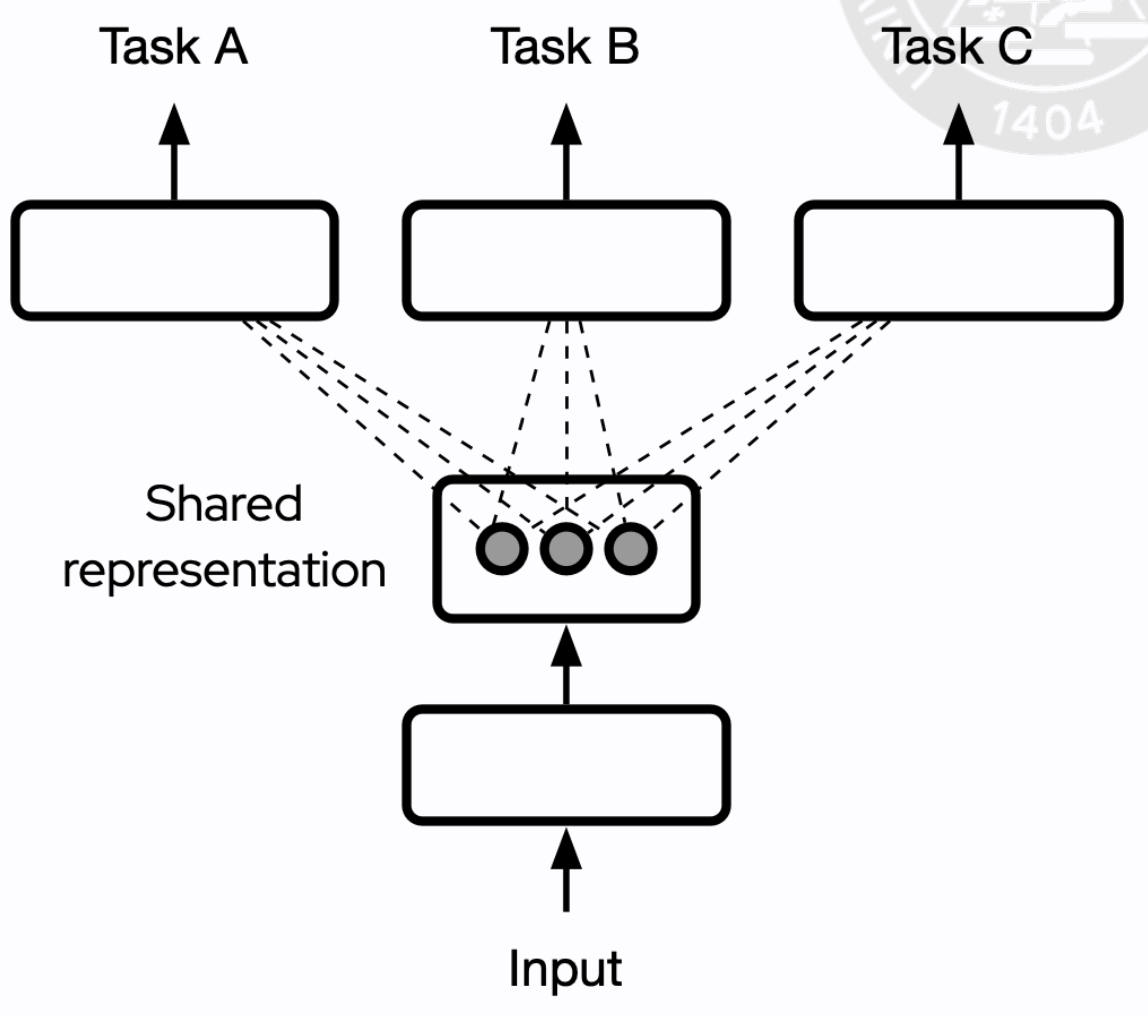
\includegraphics[scale=.5]{images/representation_learning/example.png}
  \centering
\end{figure}


E' importante notare che \textbf{cambiare la rapresentazione più rendere un problema sia più difficile che
più faicle}:
\begin{itemize}
  \item dividere due numeri può essere facile quando sono espressi in una notazione conveniente (es. notazione
  posizionale) e difficile quando non lo sono (es. numeri romani);
  \item inserire un numero nella posizione corretta è un'operazione $O(n)$ se la rappresentazione sottostante
  è una lista ordinata, è $O(\log{(n)})$ se è un albero rosso-nero.
\end{itemize}
\newpage
Una \textbf{buona rappresentazione} rende semplice il learning task successivo.


Le reti feedforward trainate con un algoritmo di apprendimento supervisionato possono essere viste come 
una sorta di esecuzione del representation learning.


Gli ultimi layer sono tipicamente semplici classificatori che possono essere molto accurati perchè il resto
della rete gli fornisce una buona rappresentazione
\begin{figure}[!h]
  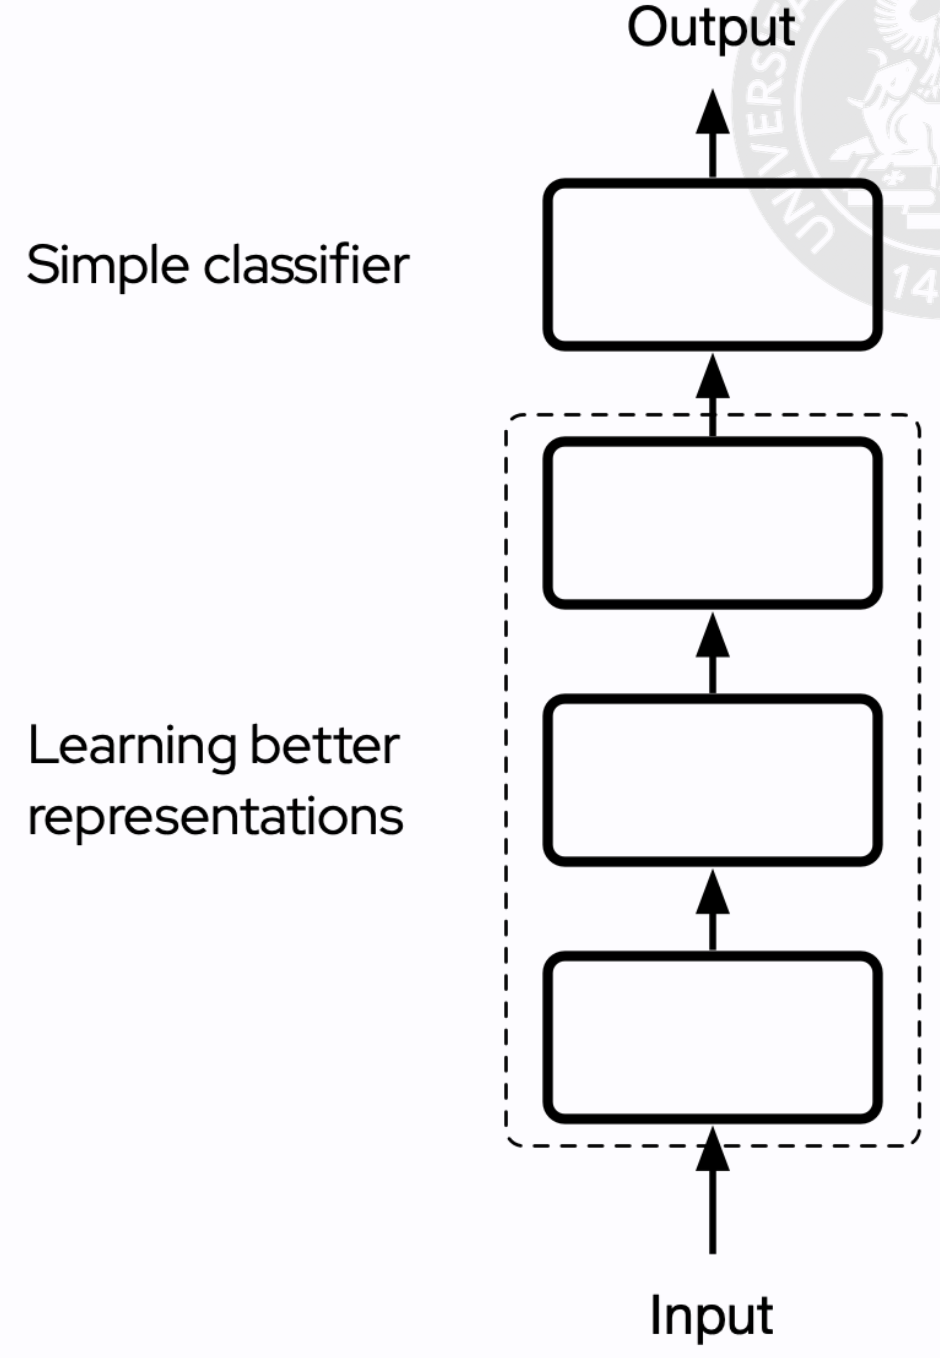
\includegraphics[scale=.5]{images/representation_learning/difficulty.png}
  \centering
\end{figure}
\newpage
\section{Greedy layer-wise unsupervised pretraining}
Illustreremo ora una tecnica di traininig inizialmente non performava bene, basata sull'idea descritta
precedentemente, ovvero \textbf{la semplificazione dell'apprendimento attraverso la costruzione di
rappresentazioni sempre migliori}.


Come al solito, è \textbf{greedy} perchè non trova l'ottimo del problema, si accontenta.
E' \textbf{layer-wise}, abbiamo una deep neural network difficile da far performare, per questo 
cerchiamo una buona rappresentazione inizialmente per il primo layer, poi per il secondo e così via.
E' \textbf{unsupervised}, infatti anche se esistono sono varianti supervised, l'orignale non lo è.
Infine è \textbf{pretrained}, anche se era pensata per essere solo un primo step nel training delle 
reti neurali. Questa tecninca è stata determinante per la rinascita delle deep neural networks.


Rappresenta una chiaro esempio di come \textbf{imparare una buona rappresentazione per un task} (apprendimento
non supervisionato, cercando di catturare la forma della distrubuzione) \textbf{a volte può essere utile per 
un altro task} (apprendimento supervisionato con lo stesso dominio in input).
\paragraph{Perchè è (stato) necessario?} Prima che le moderne tecniche venissero scoperte, le reti profonde
avevano problemi nel propagare l'informazione. Nello specifico, avevano i soliti problemi di \textbf{vanishing
ed exploding gradients}. La soluzione du quella di \textbf{dividere il processo di training generale in 
training di piccole reti} dove quei problemi sono molto meno impattanti.
\newline
\newline
La rete ha molti layer e l'idea è di allenare ogni layer attraverso \textbf{unsupervised learning}, prendendo
ogni output dei layer e \textbf{producendo come output una nuova rappresentazione dei dati}, 
la cui distribuzione è sperabilmente più utile o comunque migliore.
\begin{figure}[!h]
  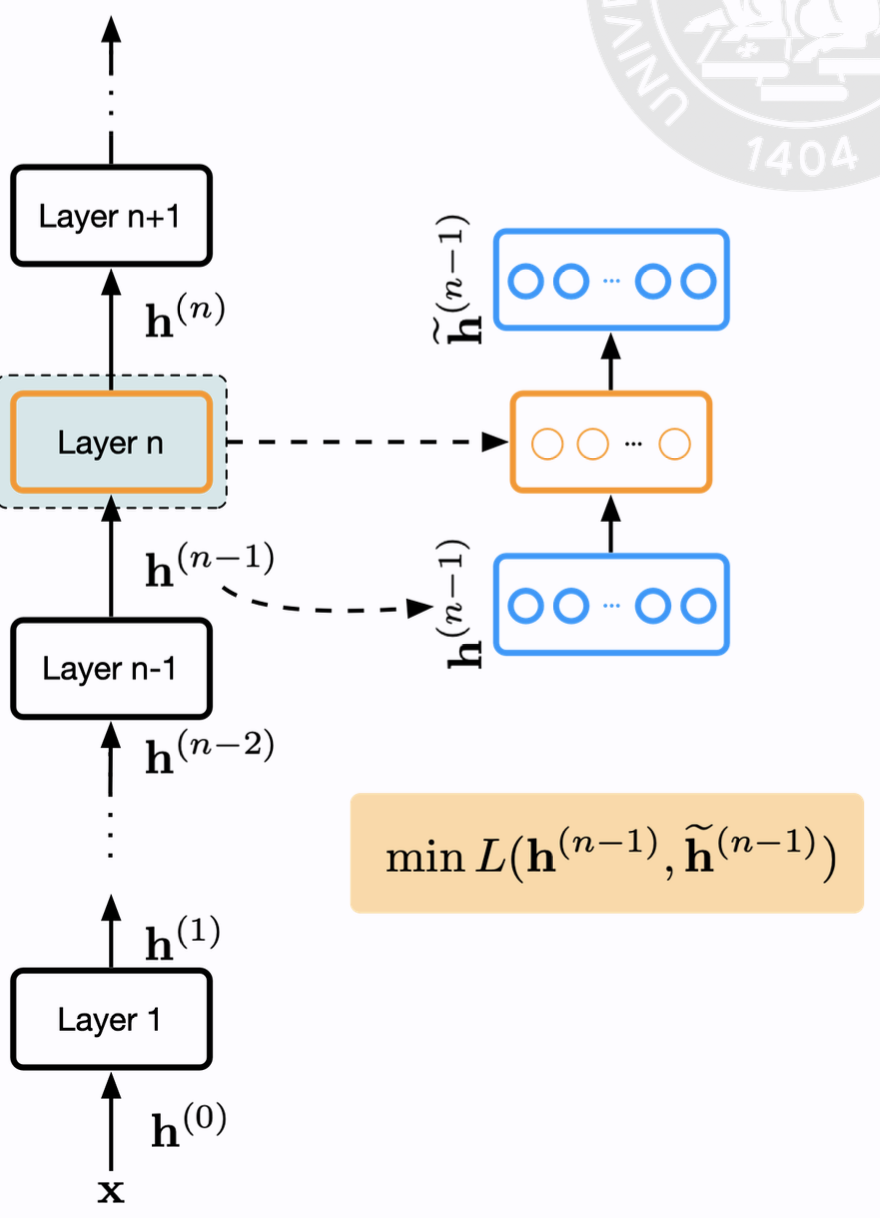
\includegraphics[scale=.4]{images/representation_learning/greedy_layer_pre.png}
  \centering
\end{figure}


Molto spesso, la procedura si basa su un \textbf{single-layer representation algorithm} come:
\begin{itemize}
  \item Restricted Boltzmann Machine;
  \item single-layer autoencoders;
  \item altre modelli che apprendono rappresentazioni latenti.
\end{itemize}
\newpage

\textbf{Un esperimento sul MNIST} 



\begin{figure}[!h]
  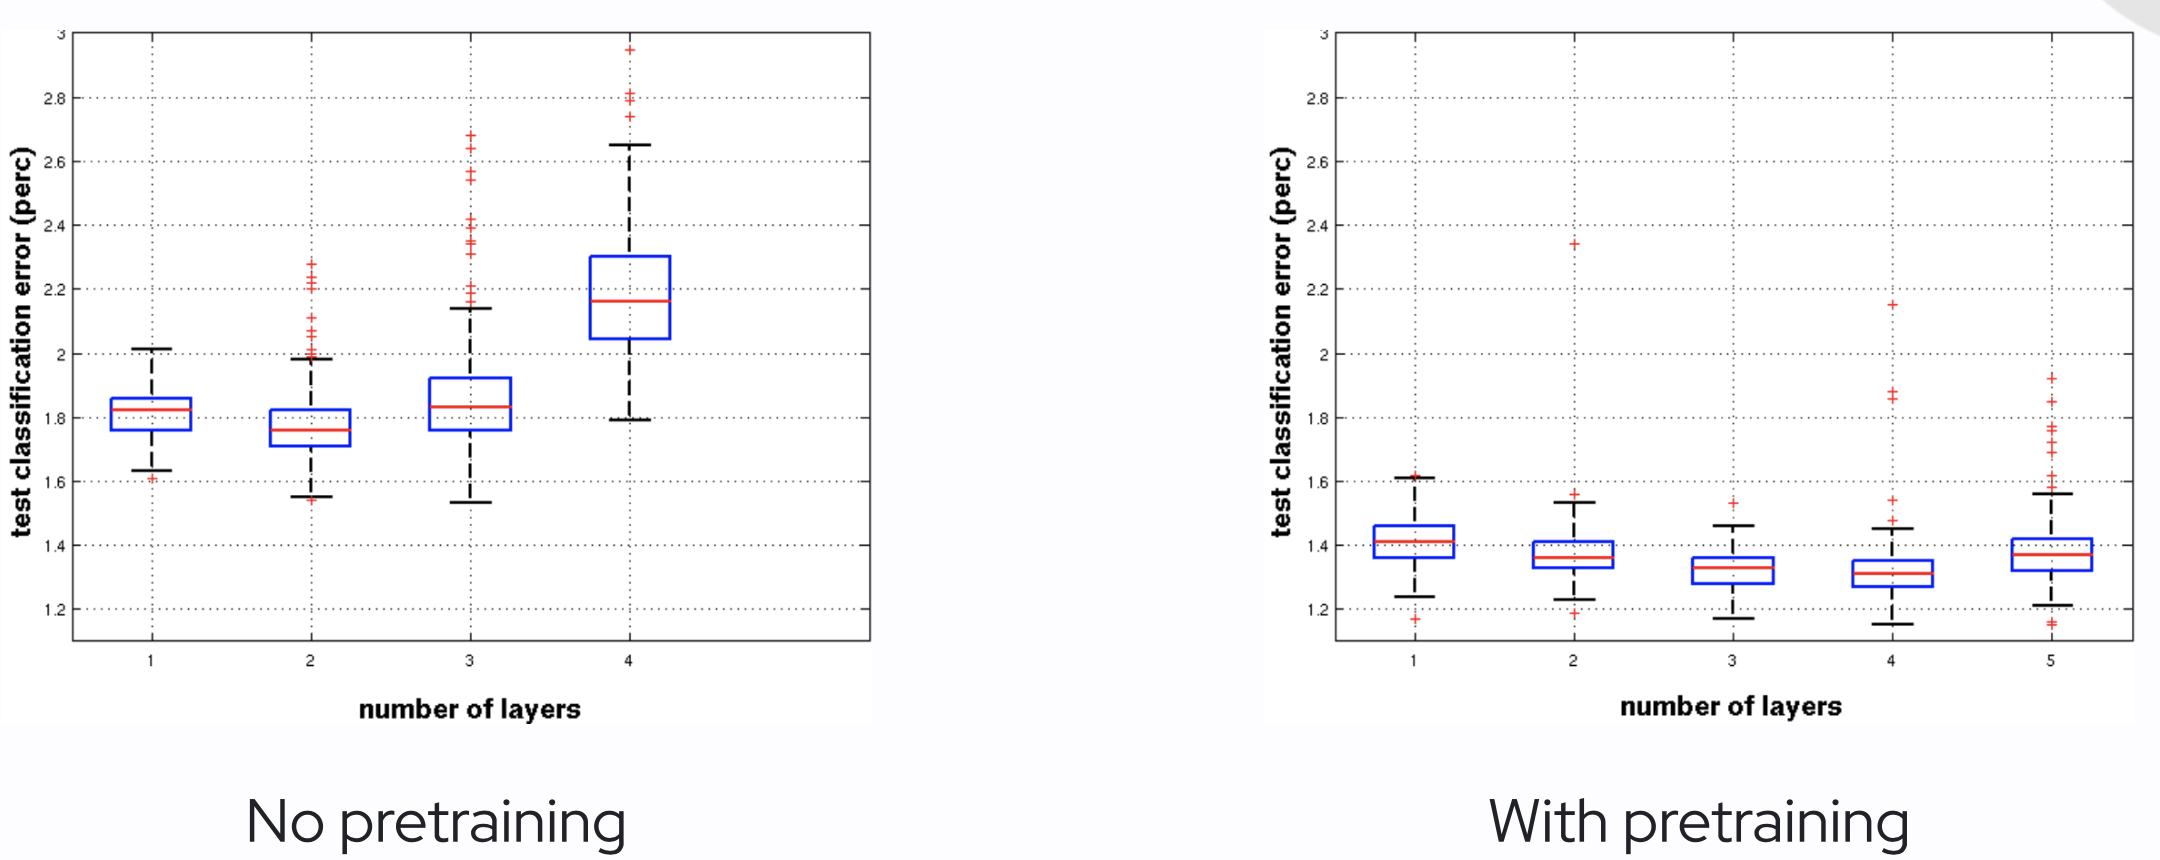
\includegraphics[scale=.45]{images/representation_learning/experiment.png}
  \centering
\end{figure}



Gli autori hanno provato questo metodo su diverse reti con un numero crescente di layer (asse x). 
L'immagine sulla sinistra mostra il box plot del test classification error di reti senza pretraining. 
\textbf{Si vede bene che l'errore cresce al crescere dei layer} e il motivo della mancanza del box plot 
nell'ultima colonna è che \textbf{gli autori non sono stati in grado di fare correttamente training della 
rete con 5 layer senza fare pretraining}.


L'immagine a destra mostra invece le stesse reti (con l'aggiunta della rete a 5 layer) su cui è stato fatto
pretraining. Si vede chiaramente che l'errore decresce al crescere del numero di layer e anche la varianza
è molto minore.
\newline
\newline
Questa procedura, il greedy layer-wise unsupervised pretraining, giocò un ruolo determinante nel 2006, quando
venne dimostrato che poteva essere utilizzata per trovare buoni punti di inizializzazione per il training di
architetture profonde.


Ad oggi sappiamo che il training delle architetture profonde è possibile e che esso non dipende necessariamente
dal greedy pretraining. In ogni caso, è fondamentale sapere che \textbf{questo approccio è stata la 
dimostrazione iniziale che questo tipo di addestramento fosse davvero possibile}.
\newpage
\subsection{Varianti}
\begin{itemize}
  \item l'algoritmo può essere utilizzato anche come inizializzazione di deep unsupervised model;
  \item è anche possibile utilizzare il greedy layer-wise \textbf{supervised} pretraining: l'idea qui è che
  mentre nella tecnica orginale estraiamo, in loop, un layer dalla rete, lo usiamo per provare a 
  ricostruire l'input, lo rimettiamo a posto, e solo alla fine facciamo il training della rete per la 
  classifiazione, qui possiamo invece far provare a classificare direttamente il layer che abbiamo estratto.
  Quindi estraiamo un layer e creiamo un nuovo problema di classificazione la cui rete è formata dal layer 
  che abbiamo estratto e da uno di classificazione. Facciamo il training di questa nuova rete e rimettiamo a 
  posto il layer che avevamo estratto. Procediamo così anche con i layer successivi, usando come input ogni
  volta l'output dei livelli precedentemente trainati.

  \item supervised e unsupervised learning contemporanei: l'idea è prendere il buono da entrambi gli approcci.
  Da un lato cerchiamo di costruire una buona rappresentazione dei dati, dall'altro cerchiamo di forzare 
  questa stessa rappresentazione in modo che vada bene anche per classificare gli esempi.
\end{itemize}

\begin{figure}[!h]
  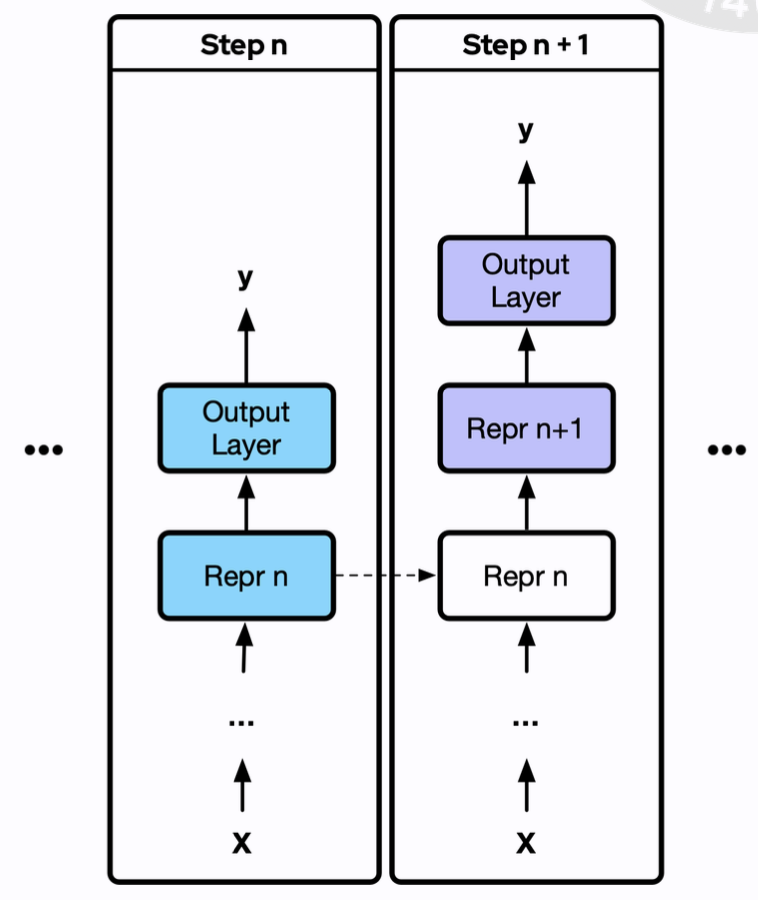
\includegraphics[scale=.4]{images/representation_learning/varianti.png}
  \centering
\end{figure}

Per quanto riguarda l'ultimo punto delle varianti, \textbf{l'integrazione permette di incorporare le costanti
imposte dall'output layer dall'outset}.
\begin{figure}[!h]
  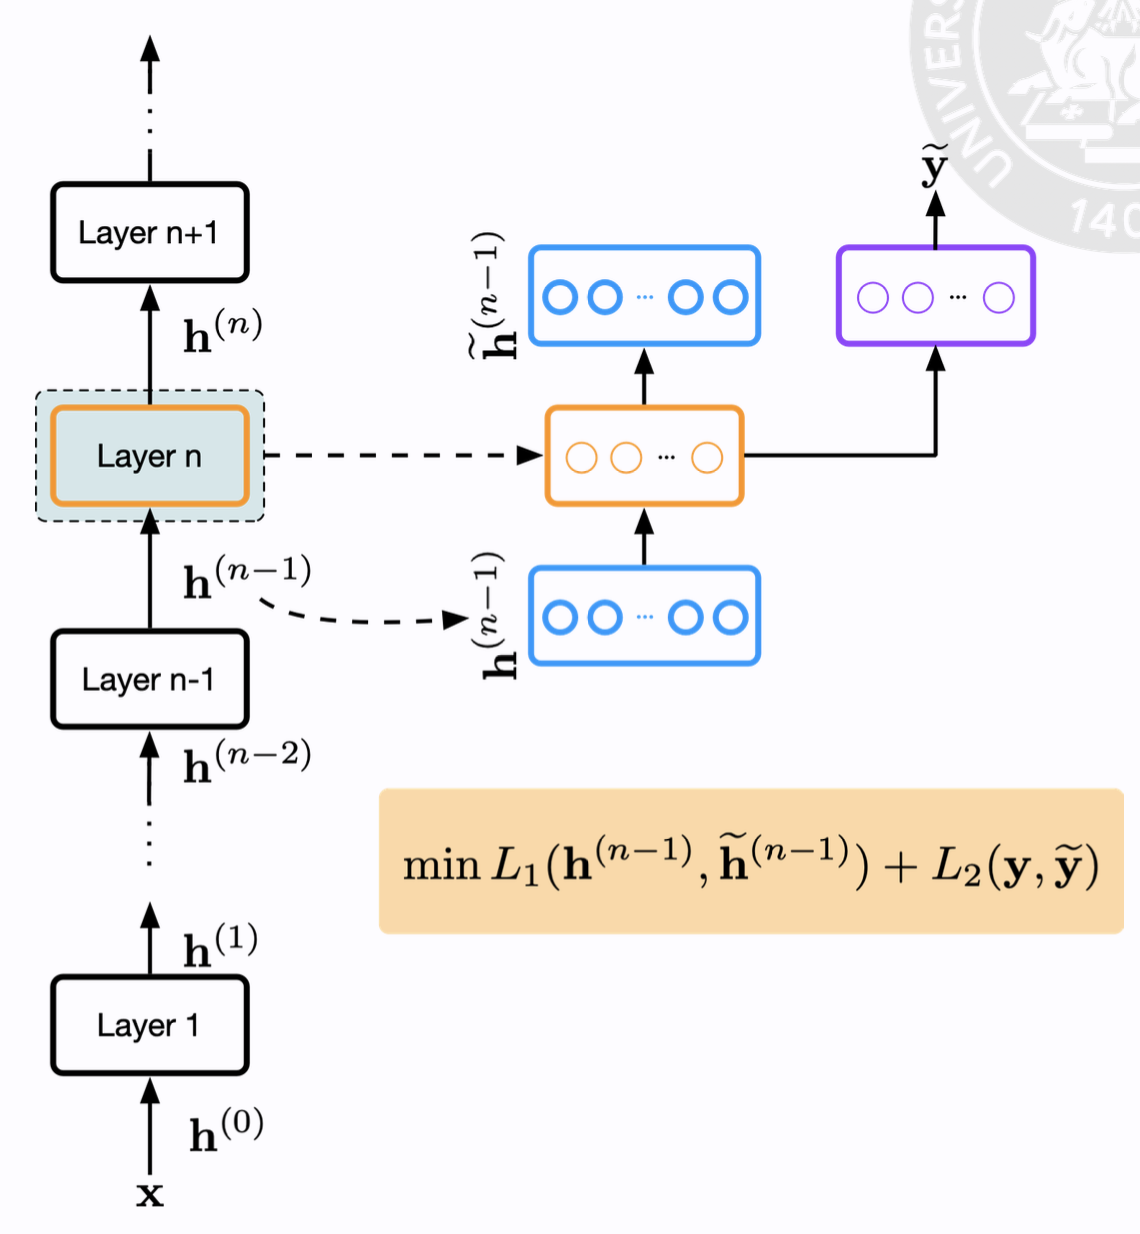
\includegraphics[scale=.4]{images/representation_learning/sup_unsup.png}
  \centering
\end{figure}
\newpage

\subsection{Perchè il pretraining non supervisionato funziona?}
Perchè cercare di ricostruire l'input può aiutare nella parte di learning? 
Le due idee alla base del funzionamento di questa procedura sono:
\begin{itemize}
  \item la \textbf{scelta degli iperparametri iniziali può avere un effetto regolarizzante significativo
  sul modello};
  \item \textbf{imparare la distribuzione di input} può aiutare ad imparare il mapping da input ad output.
\end{itemize}
\paragraph{Scelta degli iperparametri iniziali.} Inizialmente si era ipotizzato che il pretraining 
avrebbe fatto sì che il training si avvicinasse ad un minimo locale invece che ad un altro. In questo
esperimento, i ricercatori hanno utilizzato 50 reti diverse e studiato il comportamento dei parametri. 
Ogni punto nel plot rappresenta una configurazione di parametri. Nel plot a sinistra, abbiamo i parametri 
delle 50 reti composte da 2 layer, prima con pre-training e poi senza pre-training. I plot sono equivalenti,
ciò che cambia è il tipo di tecnica di riduzione della dimensionalità (sono stati mappati 10 mila parametri in 
2 dimensioni).
\begin{figure}[!h]
  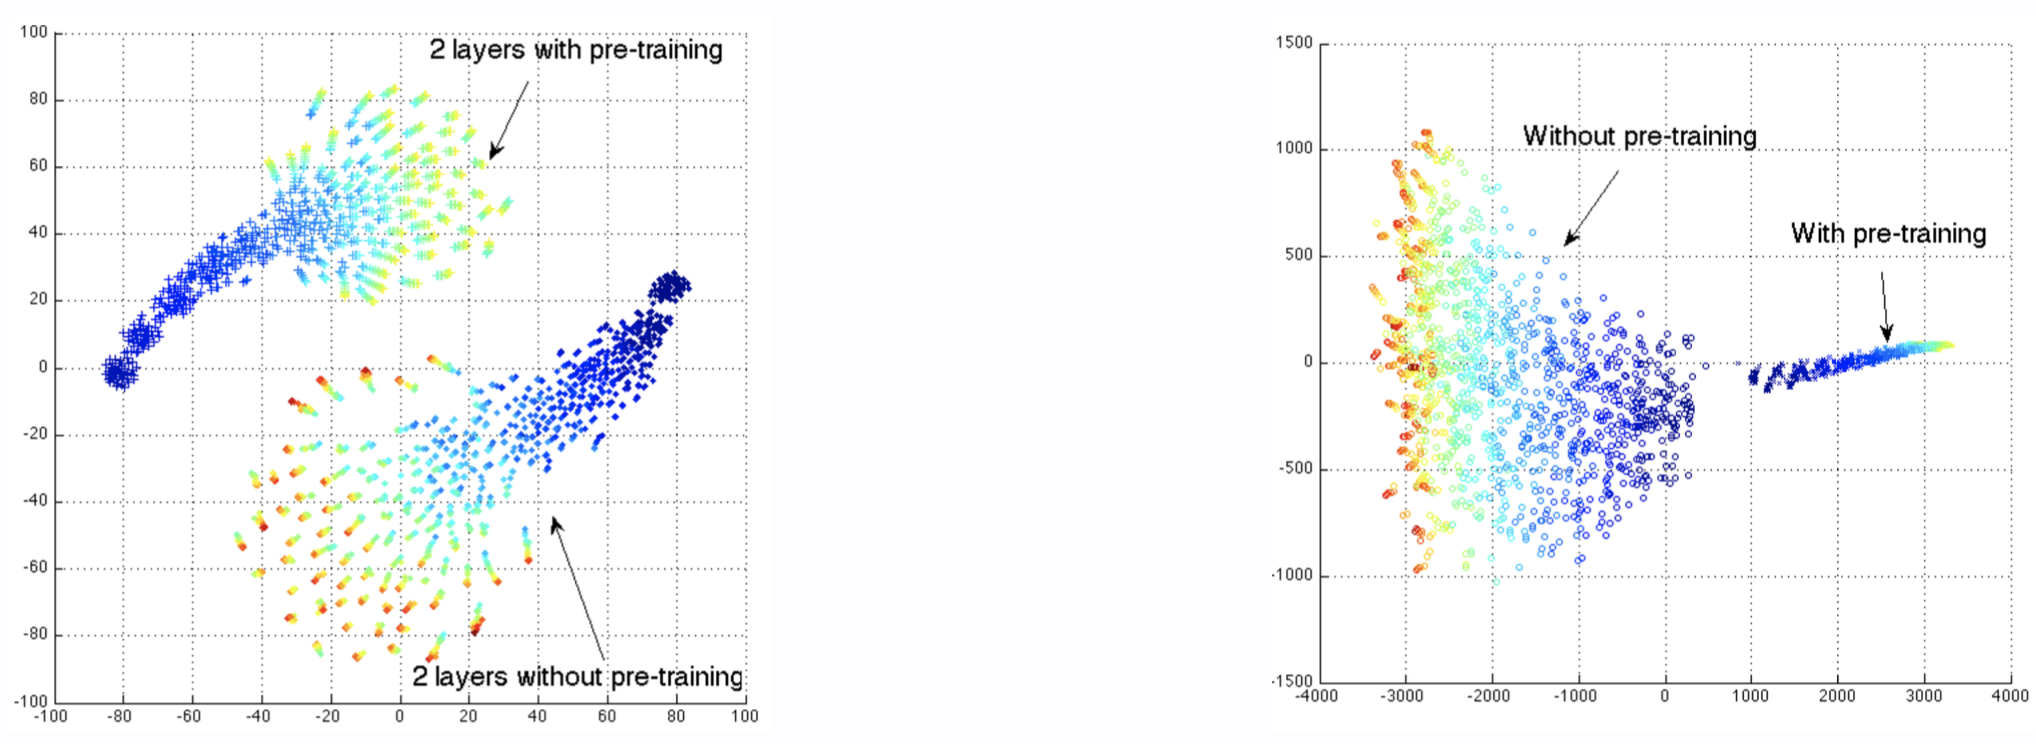
\includegraphics[scale=.5]{images/representation_learning/choice}
  \caption{plot di due differenti proiezioni di funzioni rappresentanti 50 reti trainate con e senza
  pretraining. I colori (dal blu al rosso) indicano la progressione delle iterazioni di training}
  \centering
\end{figure}
\newpage

\textbf{Alcune osservazioni:}
\begin{itemize}
  \item il training richiede più tempo senza pre-training, dal plot di sinistra si vede che le reti senza 
  pretraining hanno avuto bisogno di più epoche per convergere (punti rossi);
  \item i modelli pre-trained e non pre-trained nascono e rimangono in regioni differenti dello spazio di 
  funzione;
  \item inizialmente, tutte le traiettorie di un dato tipo si muovono insieme per poi convergere. Ciò 
  suggerisce che ogni traiettoria su muove verso un, almeno all'apparenza, diverso minimo locale;
  \begin{figure}[!h]
    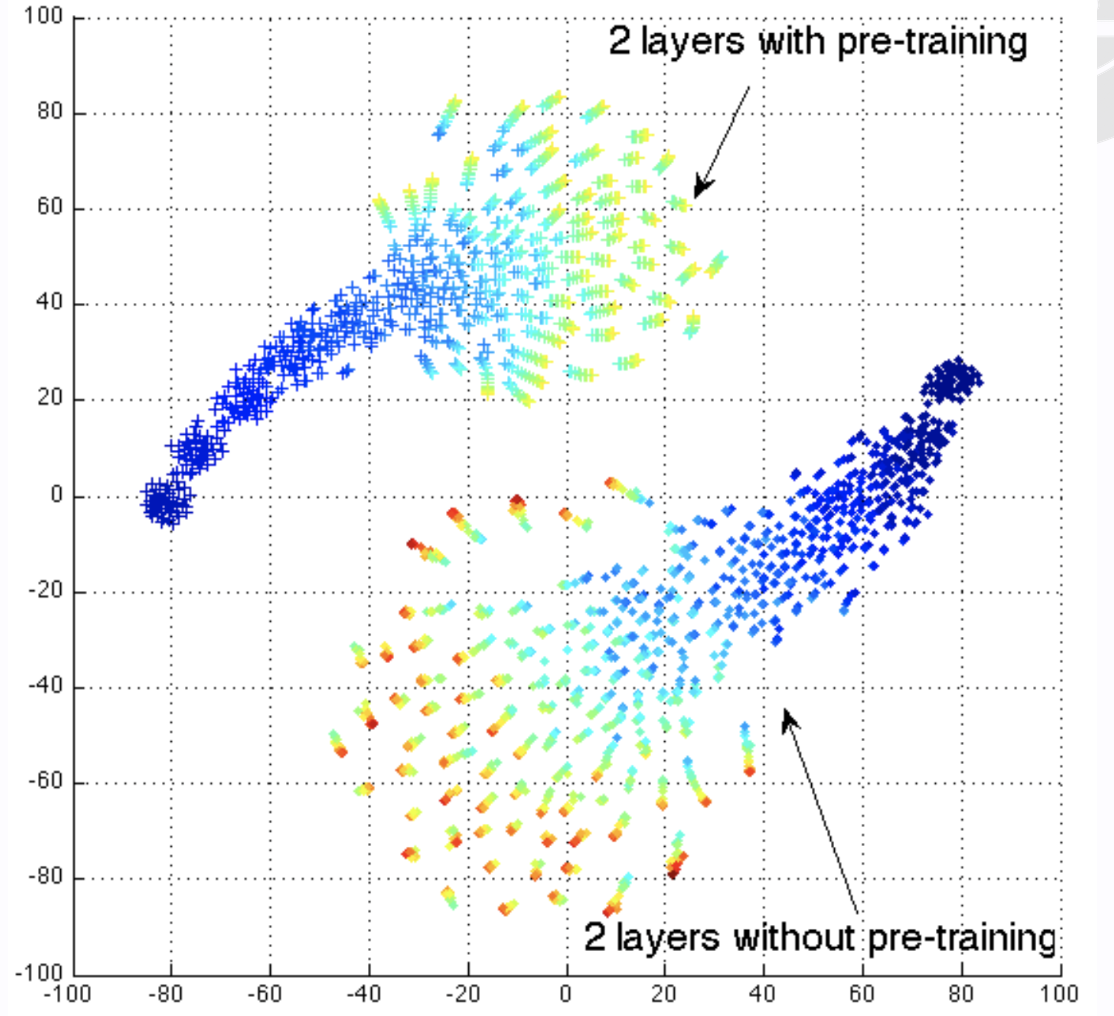
\includegraphics[scale=.35]{images/representation_learning/obs01.png}
    \centering
  \end{figure}
  \item i modelli pre-trained si trovano in una regione disgiunta e molto più piccola dello spazio rispetto
  ai non pre-trained model;
  \item le soluzioni pre-trained si somigliano molto tra loro, e questa loro autosomiglianza aumenta durante
  il training, mentre si osserva il comportamento opposto con le soluzioni pre-trained.
  \begin{figure}[!h]
    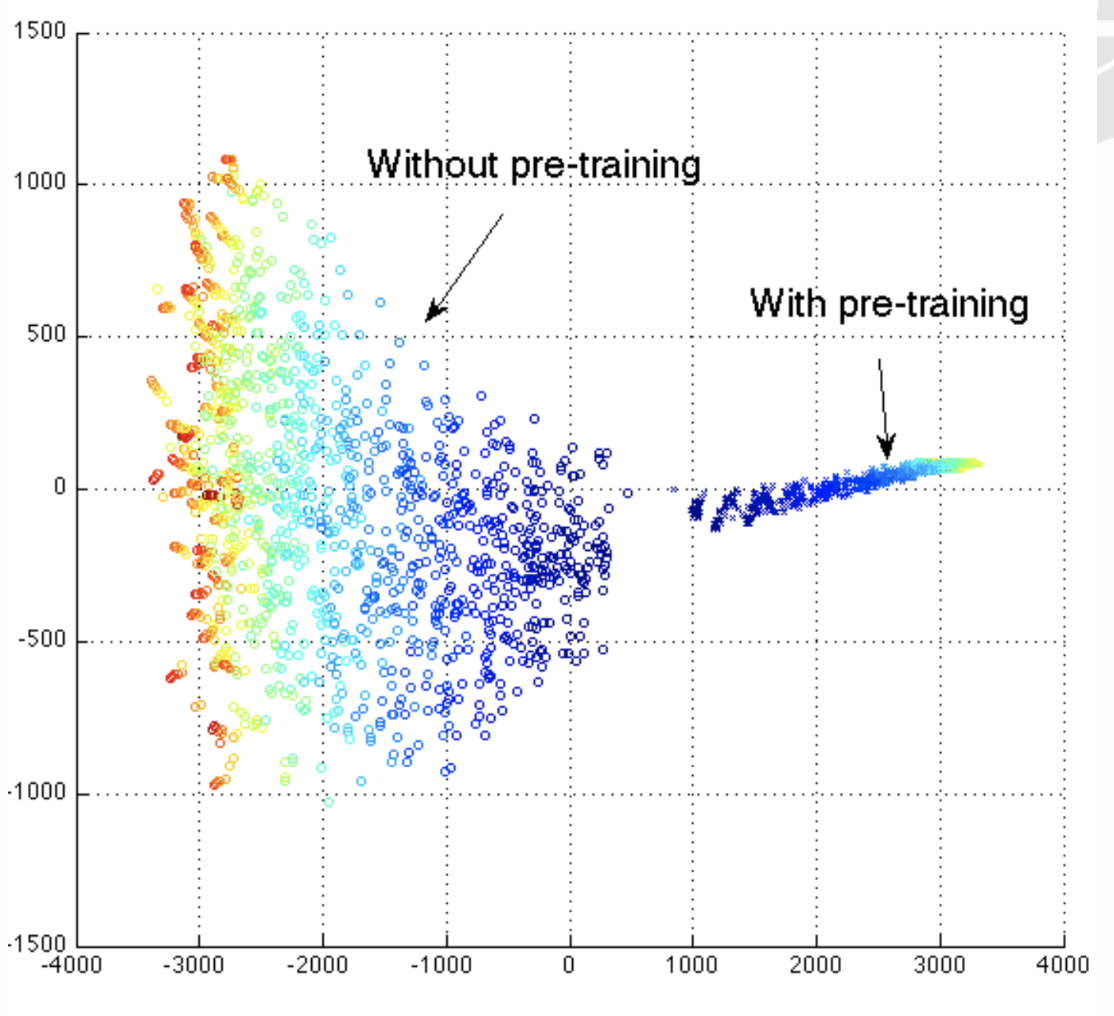
\includegraphics[scale=.35]{images/representation_learning/obs02.png}
    \centering
  \end{figure}
\end{itemize}

Uno dei problemi maggiori di questo tipo di reti, come si è visto anche nelle osservazioni all'esperimento 
precedente, era la presenza dei \textbf{minimi locali} nei loss function. Questo problema è però ormai risolto:
\textit{..recenti lavori sulla comprensione della qualità del training affermano che i punti critici 
sono più probabilmente punti di sella rispetto ad essere minimi locali spuri..\footnote{Mathematics of deep
learning}}. L'idea è che all'aumentare del numero di dimensioni (parametri), poiché \textbf{per ciascuna 
dimensione esiste una direzione di salita e una direzione di discesa}, la probabilità di 
trovare un minimo (dove tutte le direzioni sono ascendenti)diminuisce.
\newpage
\paragraph{Imparare la input distribution.}  

È ampiamente riconosciuto che in molti task le feature apprese nella fase non supervisionata possono 
essere utili anche nella fase supervisionata.
\newline
\newline
\textbf{Esempio:} apprendimento non supervisionato su immagini di automobili e motociclette.
\newline
\newline
Se siamo fortunati, il task non supervisionato può apprendere caratteristiche come la forma del
ruote che possono essere molto utili per il compito supervisionato.
\newline
I dettagli della rete possono avere un ruolo qui (ad esempio, l'utilizzo di unità di output lineari 
può forzare le rappresentazioni degli esempi a essere linearmente separabili).
\newline
\newline
La pratica dell'unsupervised pretraining è spesso utile \textbf{quando la rappresentazione originale
è povera}.
\newline
\newline
\textbf{Esempio:} il learning di work embeddings nel NLP. Per sempio nella one hot encoding le parole 
rappresentate da vettori one-hot sono particolarmente povere: due vettori diversi si trovano alla 
stessa distanza l'uno dall'altro.
\begin{figure}[!h]
  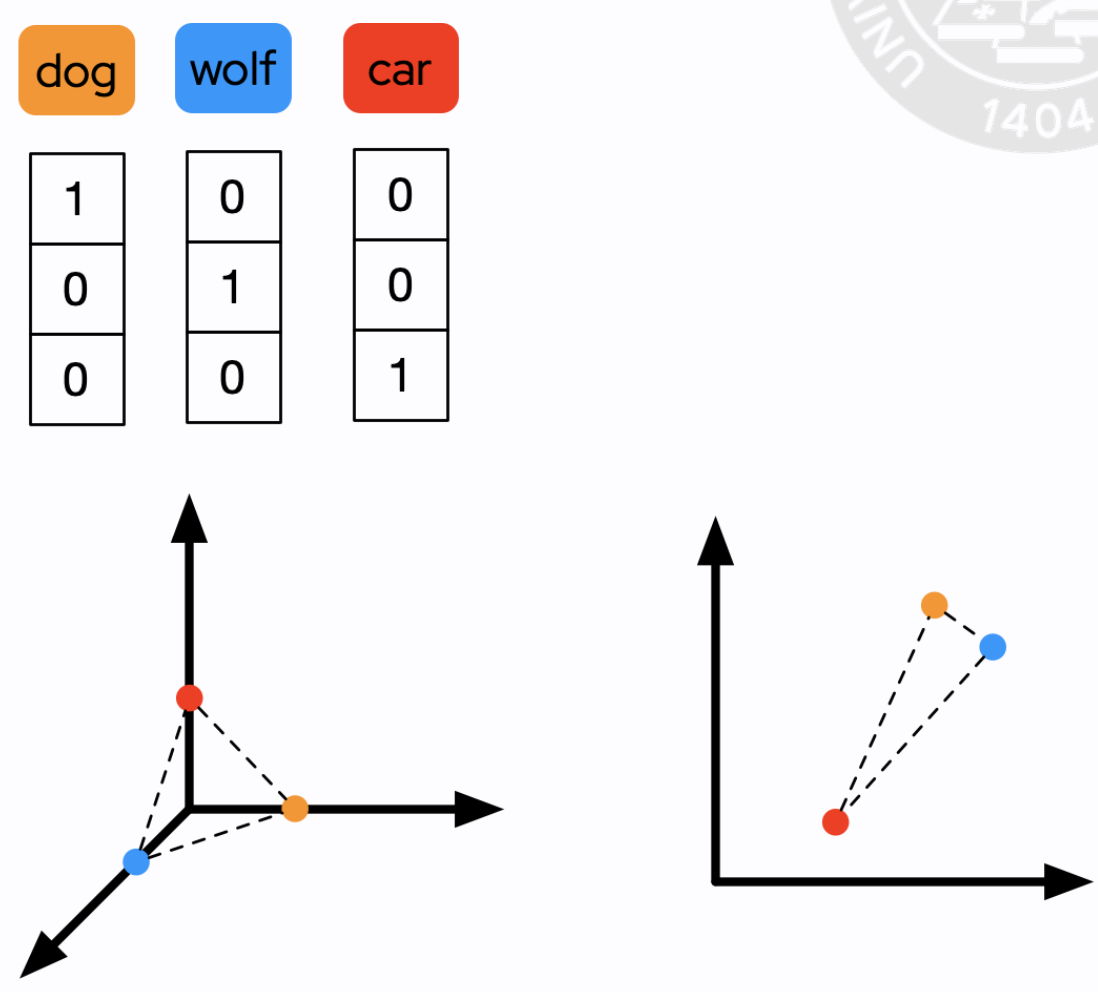
\includegraphics[scale=.4]{images/representation_learning/one_hot.png}
  \centering
\end{figure}


Inoltre considerare il pretraining non supervisionato \textbf{come un regolarizzatore} è particolarmente 
utile quando \textbf{il numero di esempi è ridotto}.
\newline
Per gli stessi motivi, è particolarmente utile anche quando \textbf{il numero di esempi senza etichetta 
è elevato}. 
\newline
È anche utile anche \textbf{quando la funzione da apprendere è estremamente complicata}.
\newline
A differenza di altri regolatori, il pretraining non supervisionato \textbf{non forza la funzione appresa 
ad essere semplice}, ma aiuta piuttosto a scoprire feature che sono utili nel task non supervisionato.
\newline
Se le vere funzioni sottostanti sono \textit{complicate \textbf{e} modellate dalle regolarità} della 
distribuzione degli input, il pretraining non supervisionato può essere un regolarizzatore più appropriato.
\paragraph{Svantaggi.} Essendo una tecnica di regolarizzazione, il pretraining non supervisionato presenta 
il problema di \textbf{essere difficile da calibrare}.
\newline
Nella maggior parte delle tecniche di regolarizzazione esiste un unico parametro che consente di impostare 
la forza della regolarizzazione.
\newline
Con l'addestramento non supervisionato, la rete viene inizializzata utilizzando il pretraining oppure no.
\newline
Inoltre, gli iperparametri della fase di pretraining devono essere regolati e questo può essere estremamente
lento.
\newpage


\section{Applicazioni del Representation Learning}
In questa sezione trattermo il \textbf{transfer leraning} e, successivamente, il 
\textbf{domain adaptation}.


Nel \textbf{transfer learning} si cerca di imparare qualcosa su una dato task per poi sfruttare ciò che si è imparato
per risolvere un task differente, diverso dal primo. Il \textbf{domain adaptation} è una variazione dell'idea 
precedente, in cui il è uno solo task, ma di cui ci sono più istanze su diversi dataset. Esistono dunque delle
differenze sul modo in cui i dati ci vengono presentati. 


In maniera più formale, il \textbf{transfer learning} e il \textbf{domain adaptation} si riferiscono alla 
situazione in cui ciò che è stato appreso in un contesto (distribuzione $P_1$) viene sfruttato per migliorare 
la generalizzazione in un altro contesto (distribuzione $P_2$).
Ciò generalizza l'idea di un \textbf{greedy pretraining} in cui le rappresentazioni trasferite si trovavano 
tra task non supervisionati e task supervisionati.
\newline
\newline
\section{Transfer Learning}
Nel \textbf{Transfer Learning} il focus è svolgere due o più compiti diversi, in cui presupponiamo che molti 
dei fattori che spiegano le variazioni in $P_1$ siano rilevanti per le variazioni che devono essere catturate
per apprendere $P_2$. 


\textbf{Esempio}: imparare a riconoscere oggetti nelle immagini di ($P_1$) gatti e cani e quindi utilizzare 
la stessa rete per riconoscere oggetti nelle immagini di ($P_2$) formiche e vespe.

\textbf{slide 32}: una delle cose più fatte è che deeper è la rappresentazione simpler è andare da un
task all'altro. il fatto interessante è che ciò sembra suggerire che deep networks cercano di astrarre.
\newline
\newline
Uno dei risultati più sorprendenti trovate è che la \textbf{profondità (depth)} sembra essere cruciale in
questo processo:


\textbf{mentre un'architettura fa uso di rappresentazioni sempre più profonde}, così la curva di 
apprendimento delle nuove categorie del secondo (transfer) setting $P_2$ migliora.
\newline
\newline
\textbf{Task:} distinguere immagini di cellule cancerogene da immagini di cellule benigne.
\begin{figure}[!h]
  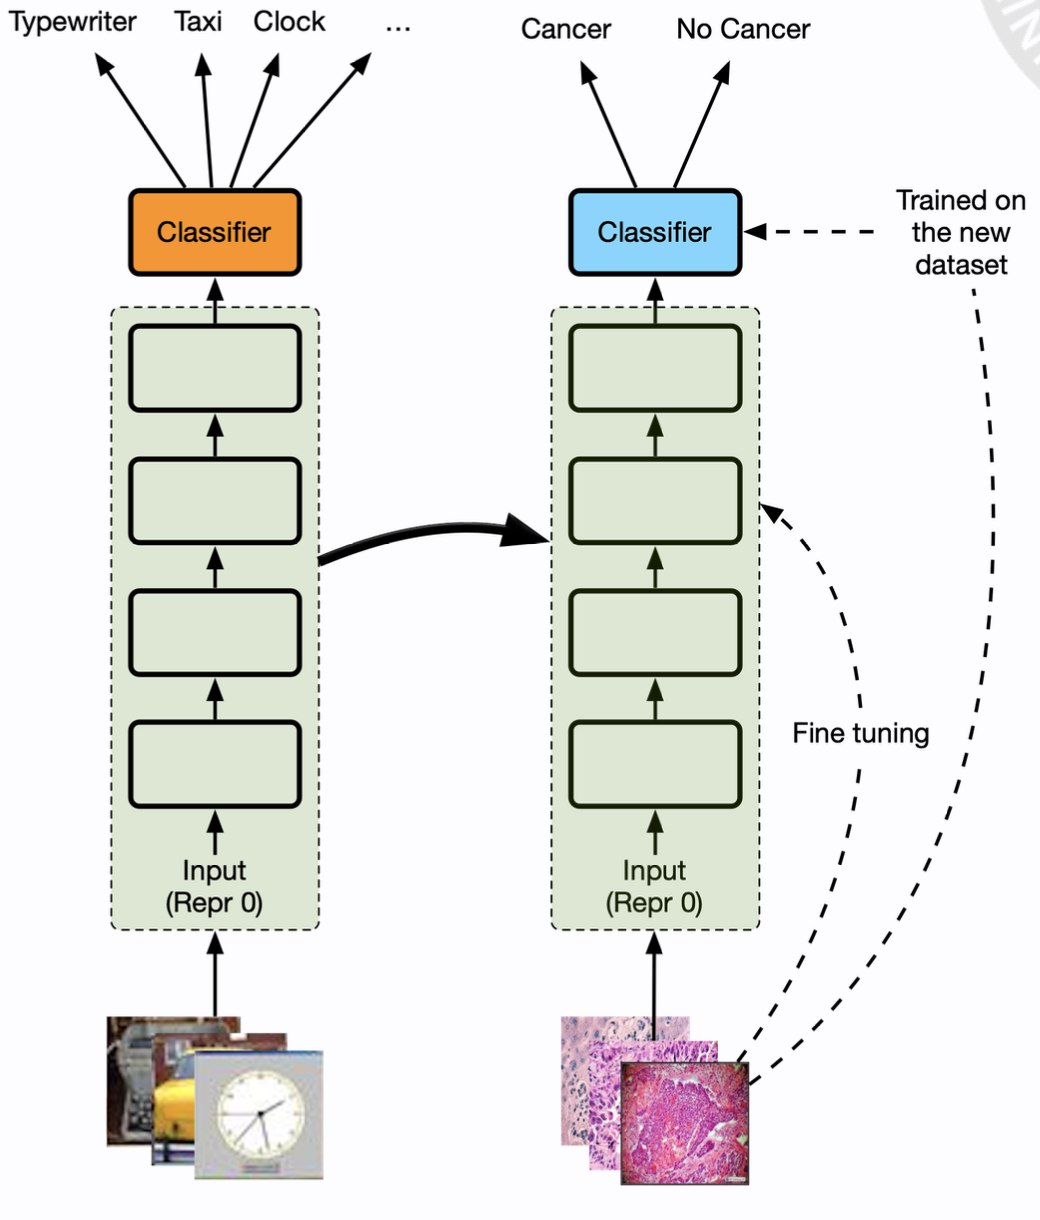
\includegraphics[scale=.5]{images/representation_learning/trans_learning.png}
  \centering
\end{figure}
\newpage
Utilizzare \textbf{pytorch} ci permette di fare transfer learning molto facilmente, 
fornisce infatti metodi per estrarre pesi e bias di un modello, di settarli in un secondo modello e di 
congelarli in modo che non vengano aggiornati in futuro.
\begin{figure}[!h]
  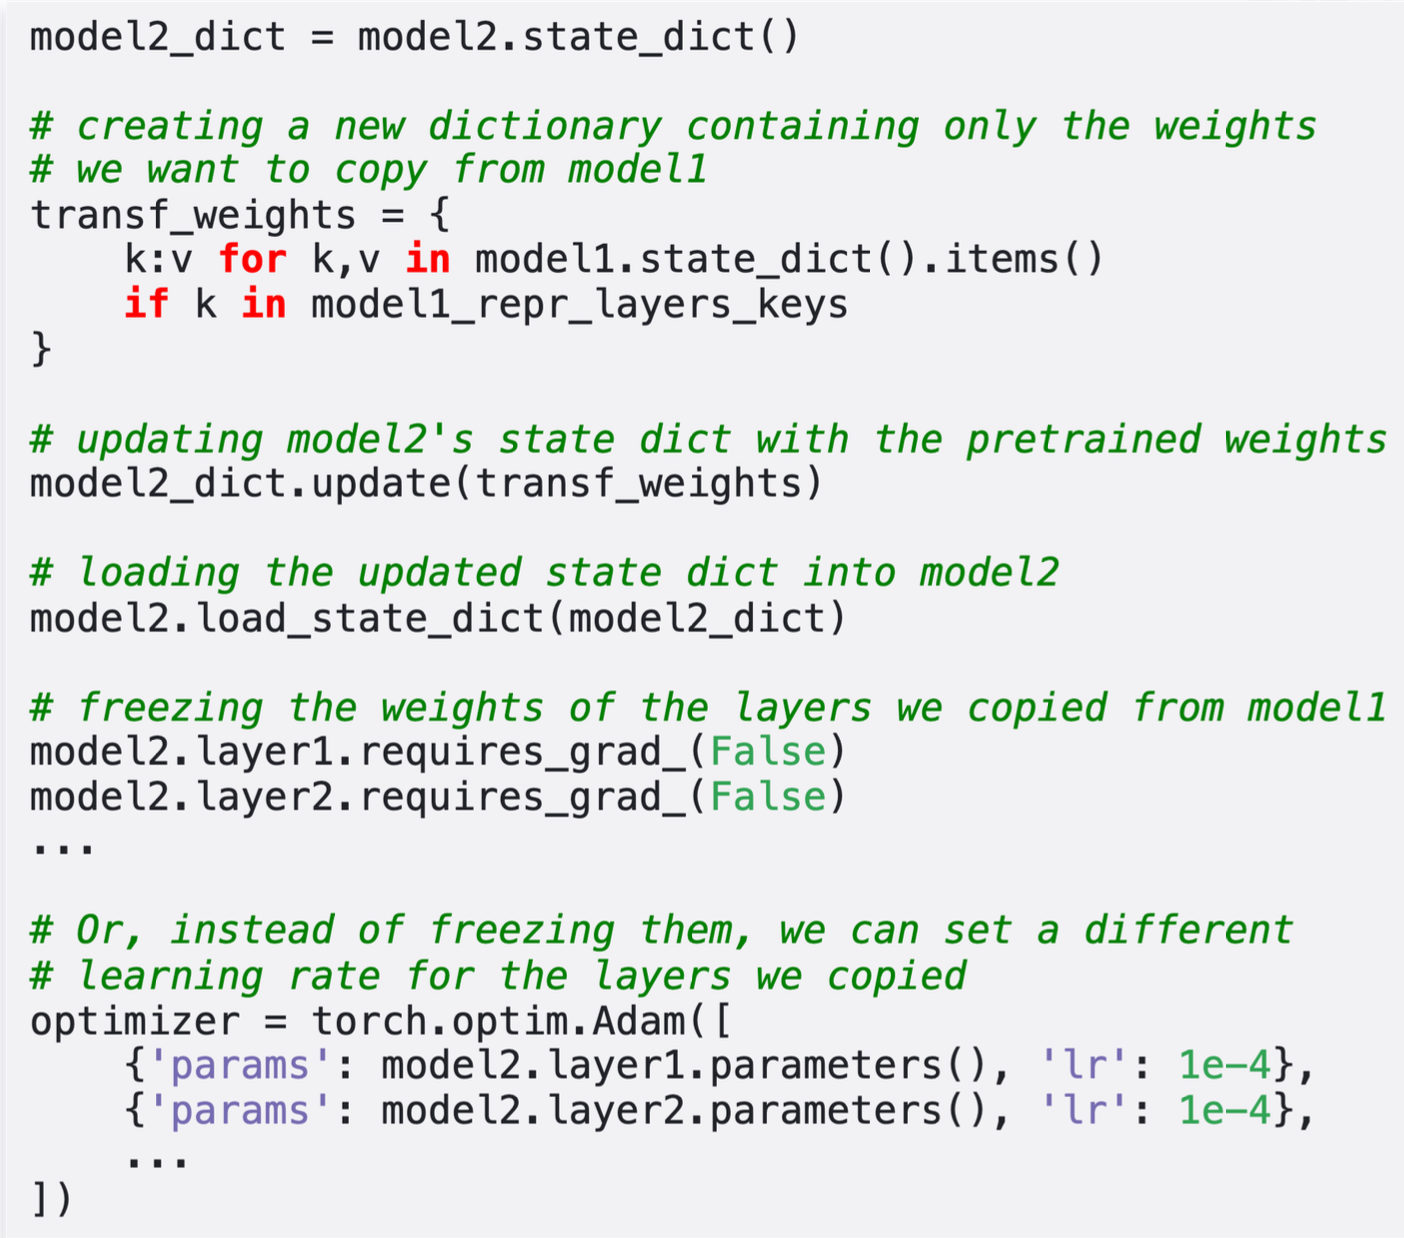
\includegraphics[scale=.5]{images/representation_learning/pytorch.png}
  \centering
\end{figure}

\newpage
In molti casi, transfer learning e domain adaptation assumono che ci sia una 
\textbf{rappresentazione comune (condivisa) che spieghi le variazioni nei dati di input}. Queste variazioni
vengono poi adattate ai vari task dai diversi output layer.


\textbf{Esempio:} image recognition.
\begin{figure}[!h]
  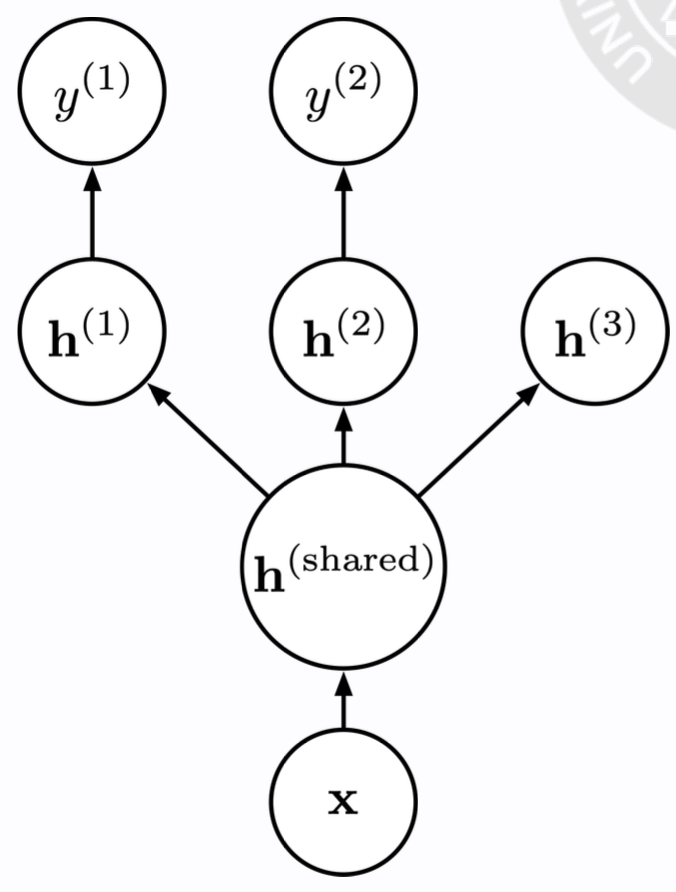
\includegraphics[scale=.5]{images/representation_learning/image_rec.png}
  \centering
\end{figure}


Ci sono però situazioni in cui è vero il contrario. Cioè situazioni in cui ciò che viene condiviso tra 
task diversi non è la semantica dell'input ma, piuttosto, la semantica degli output e degli input deve 
essere adattata per essere compatibile con essa.



\textbf{Esempio:} speech recognition.
\begin{figure}[!h]
  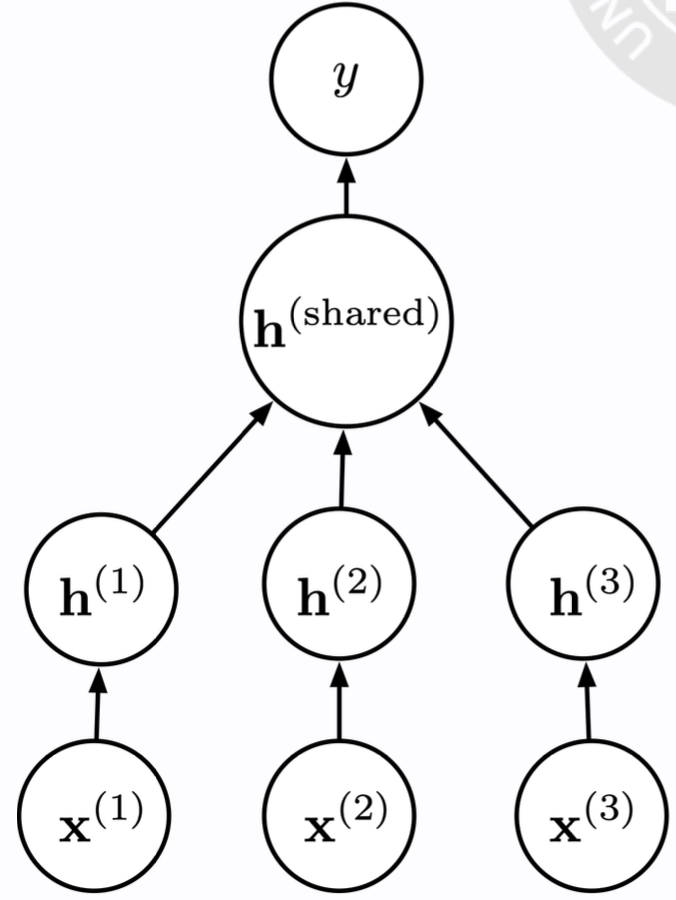
\includegraphics[scale=.5]{images/representation_learning/speech_rec.png}
  \centering
\end{figure}
\newpage
\section{Domain Adaptation}
Si tratta si domain adaptation quando abbiamo esattamente lo stesso task ma diverse istanze dello stesso in
cui il dominio è molto differente. Il caso della \textbf{sentiment analysis}: è simile allo speech recognition,
ma qui le etichette rimangono le stesse, ciò che cambia è la distribuzione dell'input. A seconda del topic
del discorso le parole utilizzate sono molto diverse ma possono essere rappresentate nello stesso modo.
\begin{figure}[!h]
  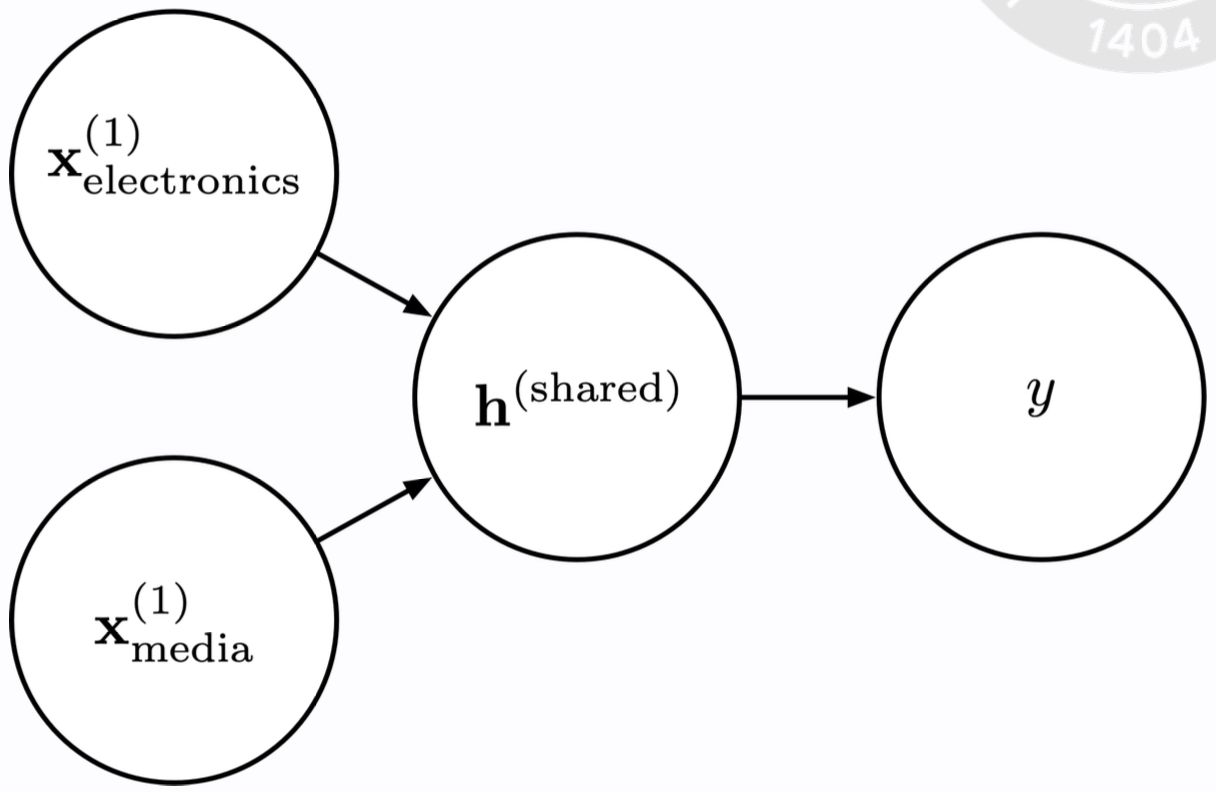
\includegraphics[scale=.3]{images/representation_learning/sentiment_an.png}
  \centering
\end{figure}

\subsection{Esempio di Domain Adaptation}
Ma come si fa domain adaptation? In un paper del 2015, gli autori cercano di prevedere le lettere da 0 a 9 
utilizzando sia il MNIST dataset che il MNIST-M. La differenza tra i due sta nel come sono rappresentate le
cifre. 
\begin{figure}[!h]
  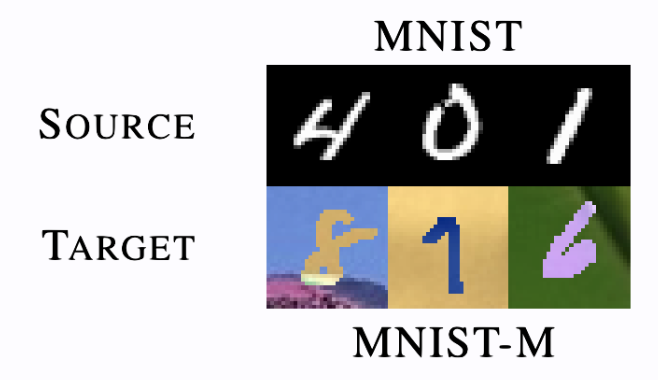
\includegraphics[scale=.4]{images/representation_learning/mnist.png}
  \centering
\end{figure}



\textbf{Task}: costruire una rappresentazione che catturi i pattern dei dati sottostanti mentre però
\textbf{ignora le sfumature specifiche del dominio}.

Viene costuita una rete la cui prima parte è di classica costruzione della rappresentazione, la seconda parte 
è invece composta da 2 pezzi diversi: quella in alto tenta di classificare le cifre normalmente (pezzo blu),
quella in basso cerca di indovinare il dominio (pezzo rosa). Tutte le volte che la rete rosa indovina 
il dominio, la rete blu, che ha costruito quella rappresentazione, viene penalizzata. Questo perchè non ha 
impedito alla rete rosa di indovinare. L'obiettivo è \textbf{la corretta previsione da parte della rete rosa}. 
La rete rosa viene invece penalizzata quando non indovina. In questo modo si sta facendo \textbf{gradient
ascend} al posto di \textbf{descend} nella seconda parte della rete. Un aspetto interessante è che tutto può
essere fatto all'interno di un singolo training loop. Si può inoltre usare una loss che contenga tutte 
le parti e flippare la loss della seconda parte della rete. 
\begin{figure}[!h]
  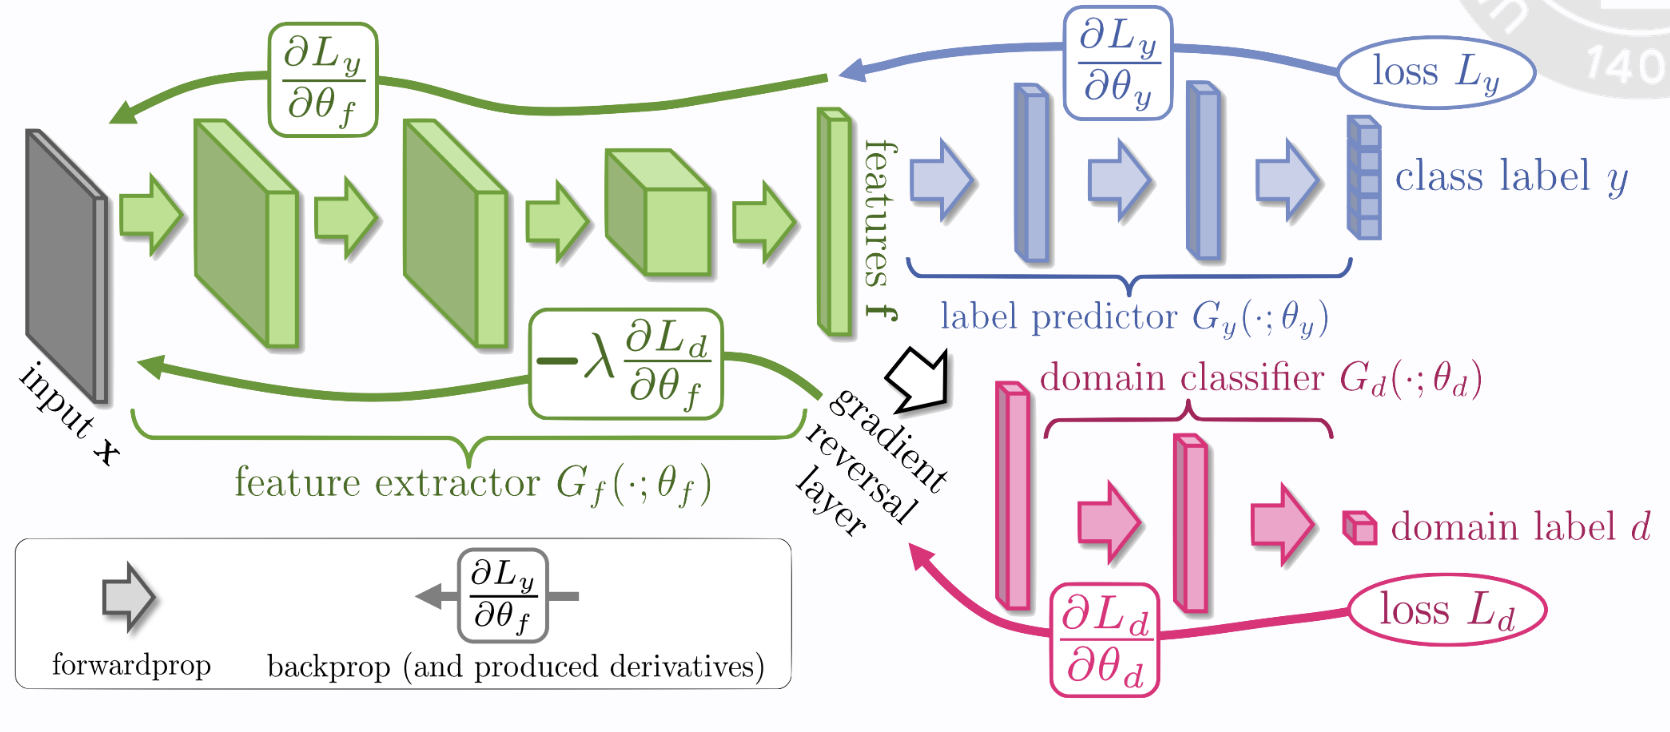
\includegraphics[scale=.3]{images/representation_learning/dom_ad_ex01.png}
  \centering
\end{figure}
\newpage

\section{Concept Drift}
Il concept drift si verifica quando il concetto alla base della distribuzione dei dati si sposta nel tempo. 
Un modello appreso in un dato momento necessita, quindi, di essere aggiornato per tenere conto del data shift
nel tempo. 


Come nei casi precedenti, l'idea è quella di sfruttare i dati di un dato setting (la distribuzione prima 
del drift) per ottenere un vantaggio in un altro contesto (la distribuzione dopo il drift).


Il concept drift è un problema ampio e molto studiato in machine learning.
\begin{figure}[!h]
  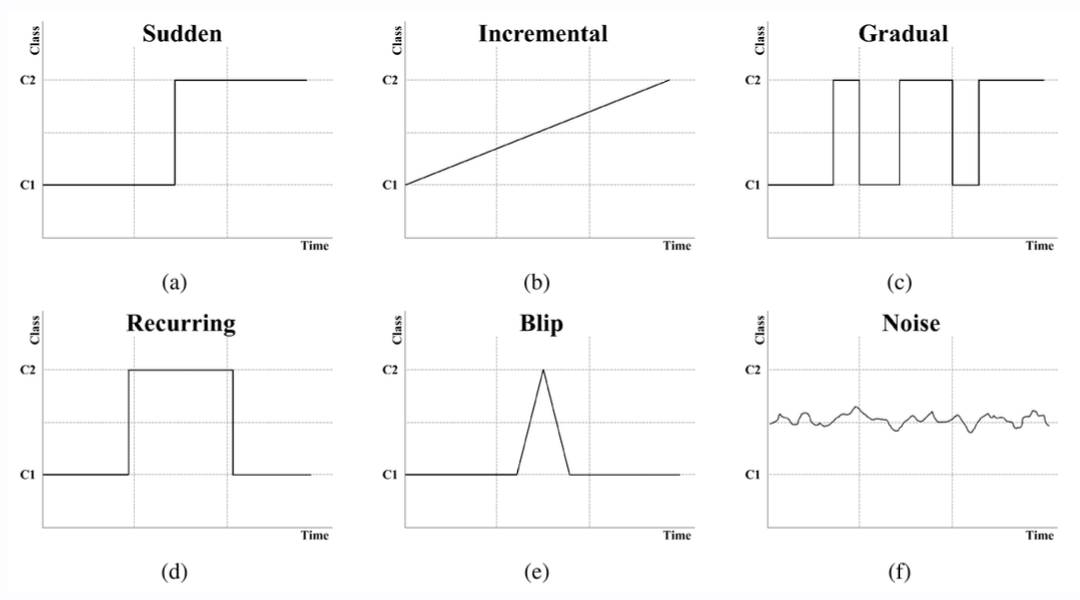
\includegraphics[scale=.5]{images/representation_learning/concept_drift.png}
  \centering
\end{figure}
\newpage
\section{One e Zero-Shot Learning}
\subsection{One-Shot Learning}
Questo è un caso estremo di transfer learning, un learning settings estremo. Si tratta di un learning setting 
particolare in cui si ha un solo esempio per classe. L'obbiettivo è quindi adattare a riconoscere una classe 
a partire da un solo esempio. In realtà è quasi impossibile partendo da zero, ma se abbiamo un modello che sa
almeno dividere gli esempi in 2 diverse regioni nello spazio rappresentazionale, è molto probabile che quando
arriva un nuovo esempio esso verrà collocato in un punto dello spazio non utilizzato prima, essenzialmente 
utlizzandolo come prototipo di una nuova classe.
\begin{figure}[!h]
  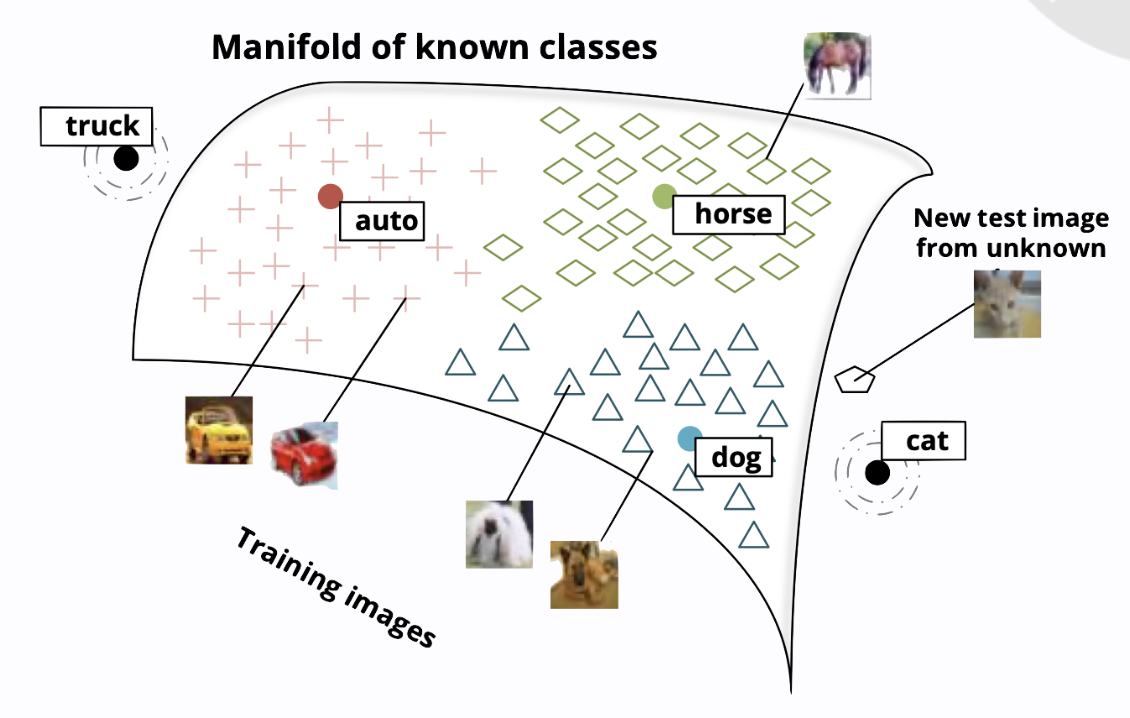
\includegraphics[scale=.5]{images/representation_learning/one_shot.png}
  \centering
\end{figure}
\subsection{Zero-Shot Learning}
\textbf{slide 41}: La versione più estrema del One-Shot è lo Zero-Shot Learning. In questo caso non si ha
nemmeno un singolo esempio. E' sostanzialmente ciò chge fa chatgpt: a partire da un pezzo di testo dato, 
lo riesce riscrivere in un certo modo specificato in input. Il punto è viene fornita solo la descrizione 
su come si vuoe che il task venga risolto. Da qui si capisce che ChatGPT ha una buona rappresentazione 
delle cose nello spazio e che riesce ad utilizzarla bene.
\newpage
\section{Semi-Supervised Learning e Causality}
L'apprendimento semi-supervisionato è un setting in cui ci viene fornita una grande quantità di esempi, 
ma solo pochi di essi sono etichettati. Il compito è sfruttare gli esempi senza etichetta per eseguire 
meglio il task supervisionato. La domanda è: qual è il miglior classificatore per i due punti nella slide?
\begin{figure}[!h]
  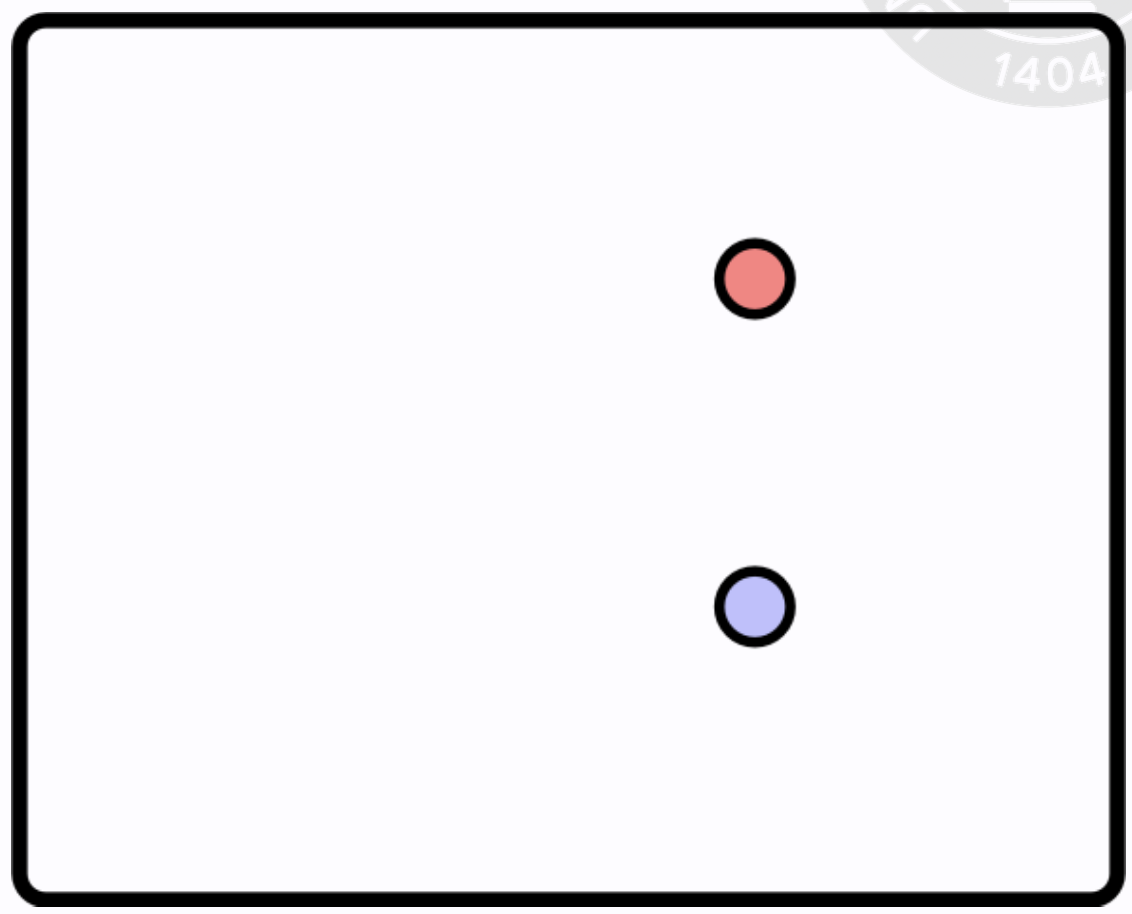
\includegraphics[scale=.25]{images/representation_learning/ssl01.png}
  \centering
\end{figure}


Verosimilmente è una linea al centro del grafico:
\begin{figure}[!h]
  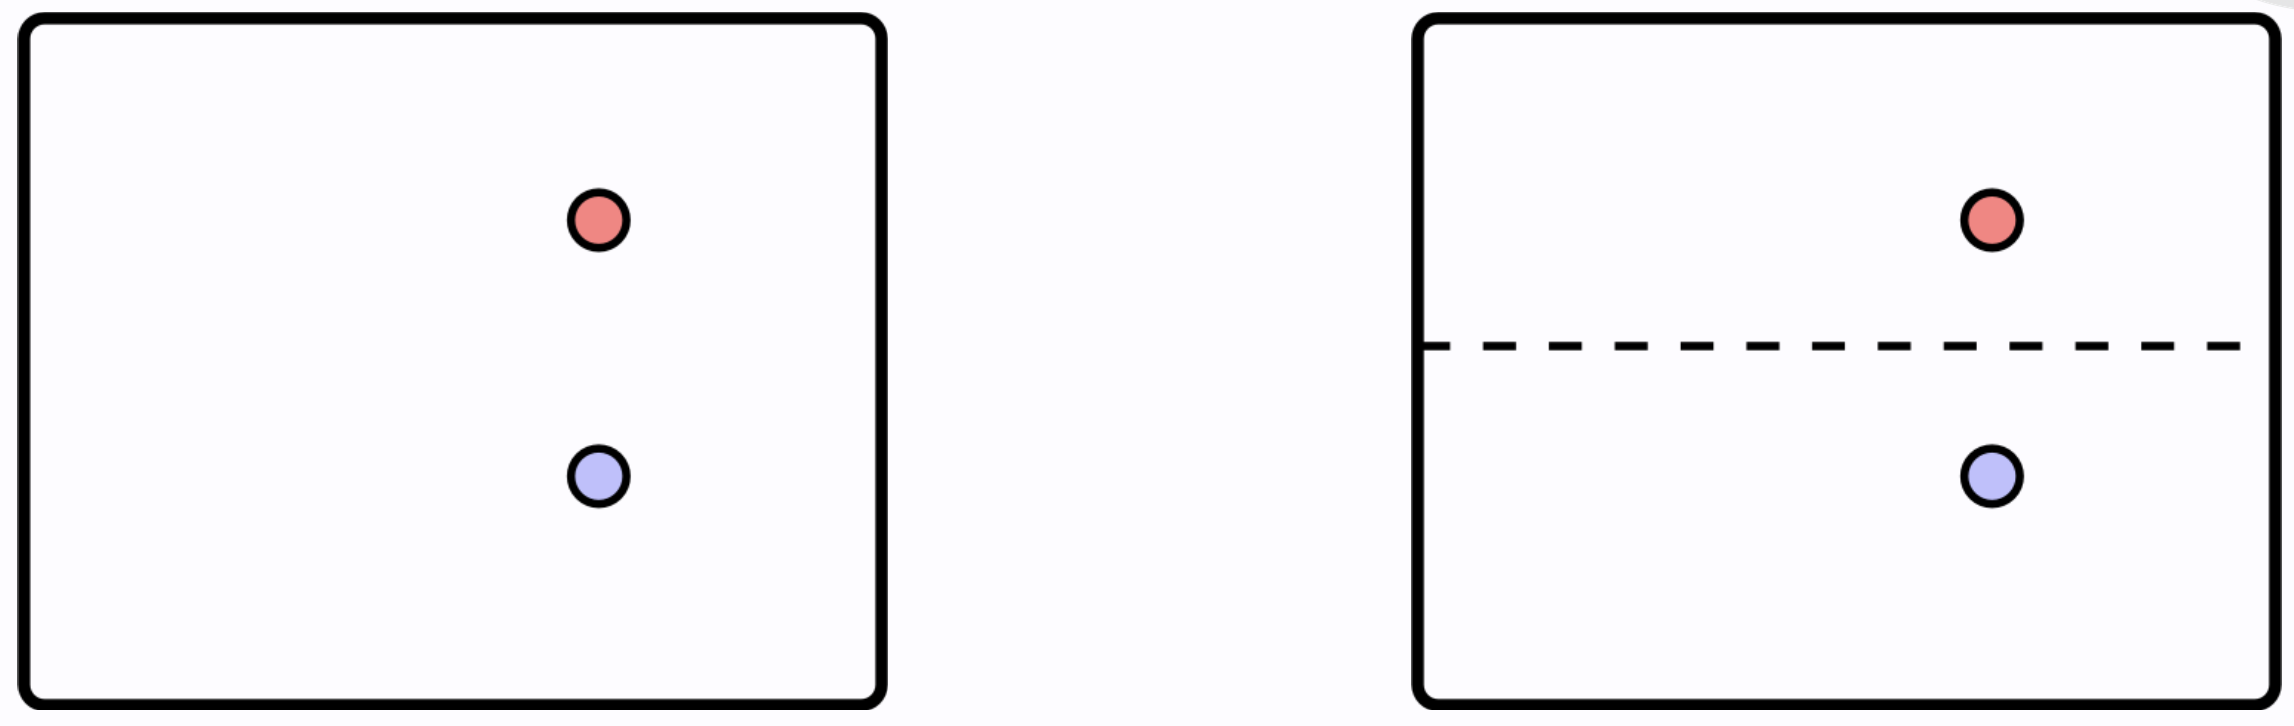
\includegraphics[scale=.3]{images/representation_learning/ssl02.png}
  \centering
\end{figure}


In questo caso, invece?
\begin{figure}[!h]
  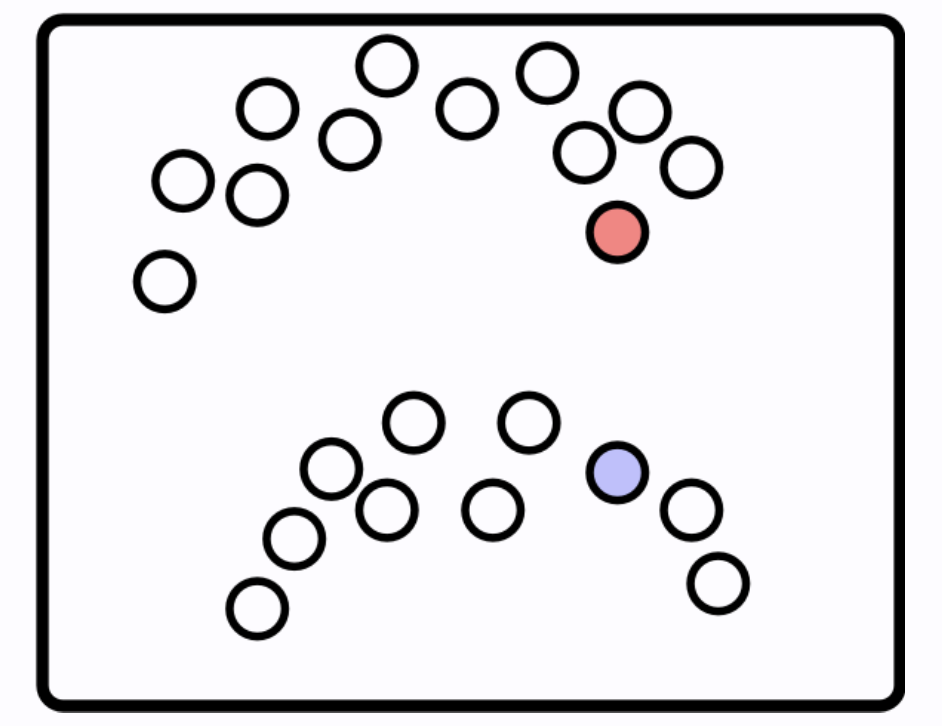
\includegraphics[scale=.3]{images/representation_learning/ssl03.png}
  \centering
\end{figure}


La migliore ipotesi è una parabola:
\begin{figure}[!h]
  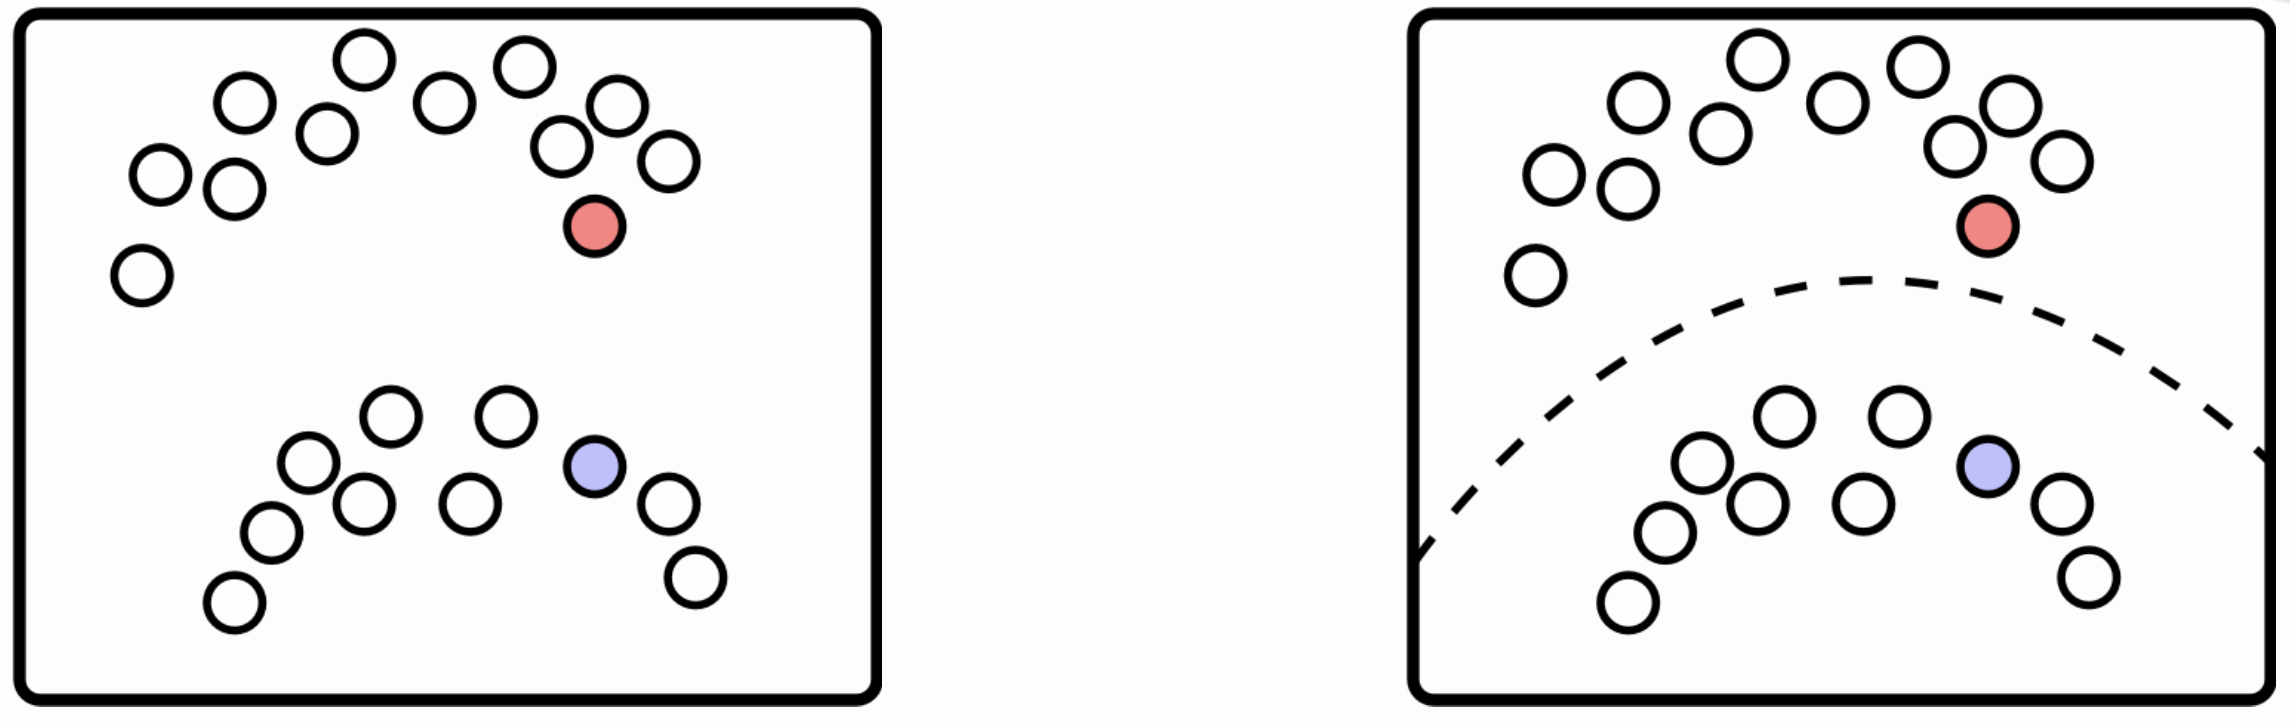
\includegraphics[scale=.3]{images/representation_learning/ssl04.png}
  \centering
\end{figure}
\newpage
\subsection{Cosa rendere una rappresentazione migliore di un'altra?}
\textbf{Ipotesi:} una \textbf{rappresentazione ideale} è una rappresentazione in cui le \textbf{feature}
all'interno della rappresentazione corrispondono alle \textbf{cause sottostanti} dei dati osservati


L'idea è di trovare quei fattori causali. 
\newline
\newline
L'\textbf{ipotesi di causalità} è alla base di gran parte della ricerca motivata dall'idea che districare 
i fattori causali in $p(x)$ potrebbe essere un buon passo verso imparare $p(y|x)$ e \textbf{motiva l'approccio
SSL}.
\newline
\newline
Prima di procedere con questa idea, ricordiamo che non sempre questo approccio funziona: per esempio
a volte SSL fallisce perchè l'apprendimento non supervisionato di $p(x)$ non è d'aiuto per apprendere $p(y|x)$.
\begin{figure}[!h]
  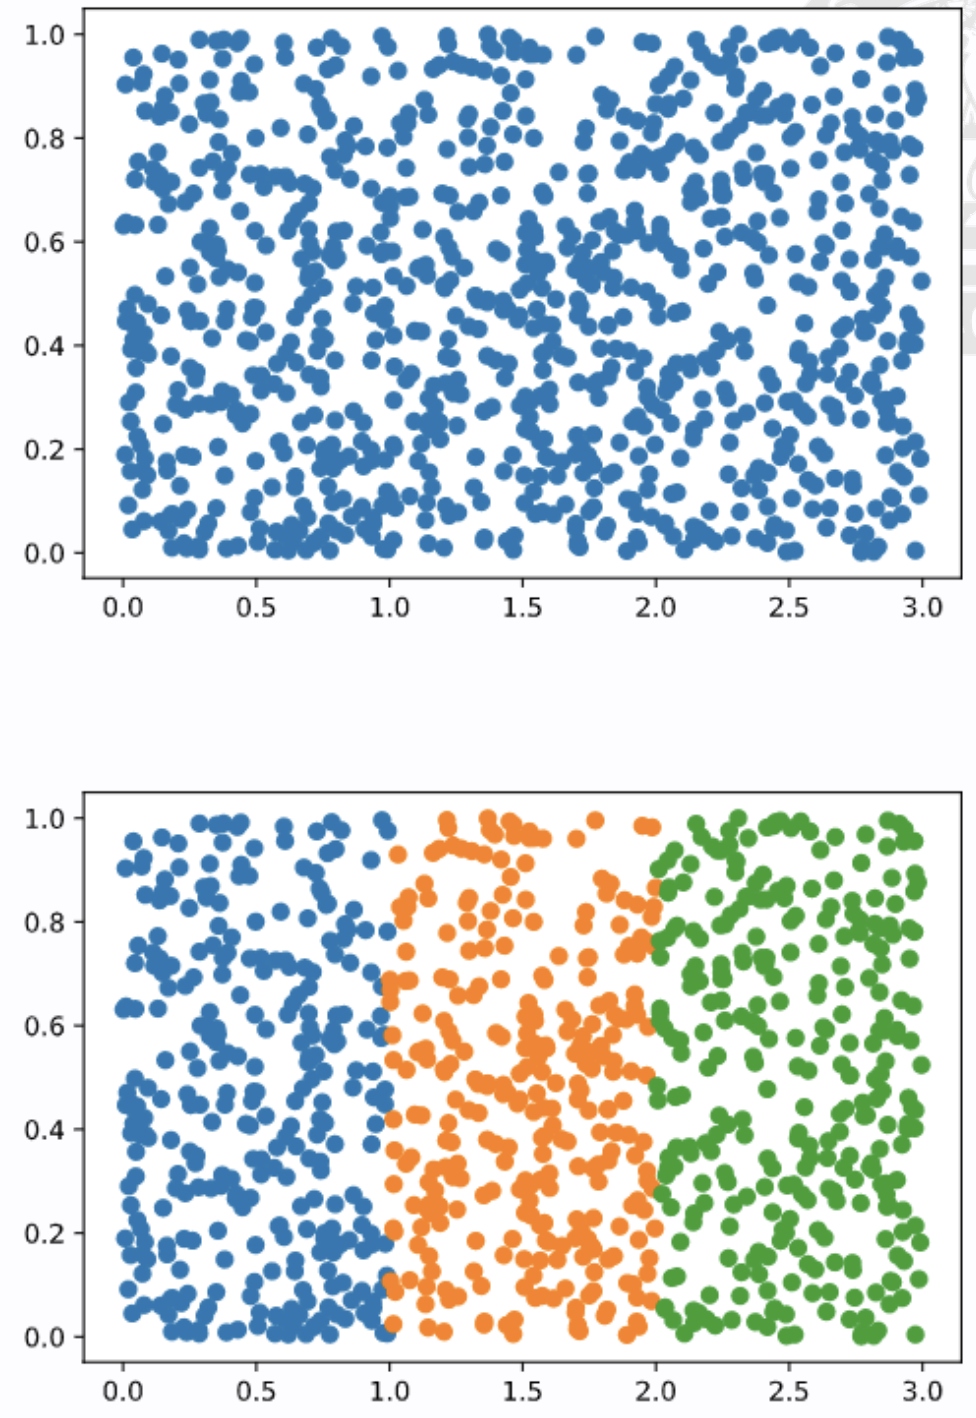
\includegraphics[scale=.3]{images/representation_learning/failure.png}
  \centering
\end{figure}


Altre volte, $y$ è tra le cause salienti di $p(x)$. In questi casi apprendere $p(x)$ può essere molto utile.
\begin{figure}[!h]
  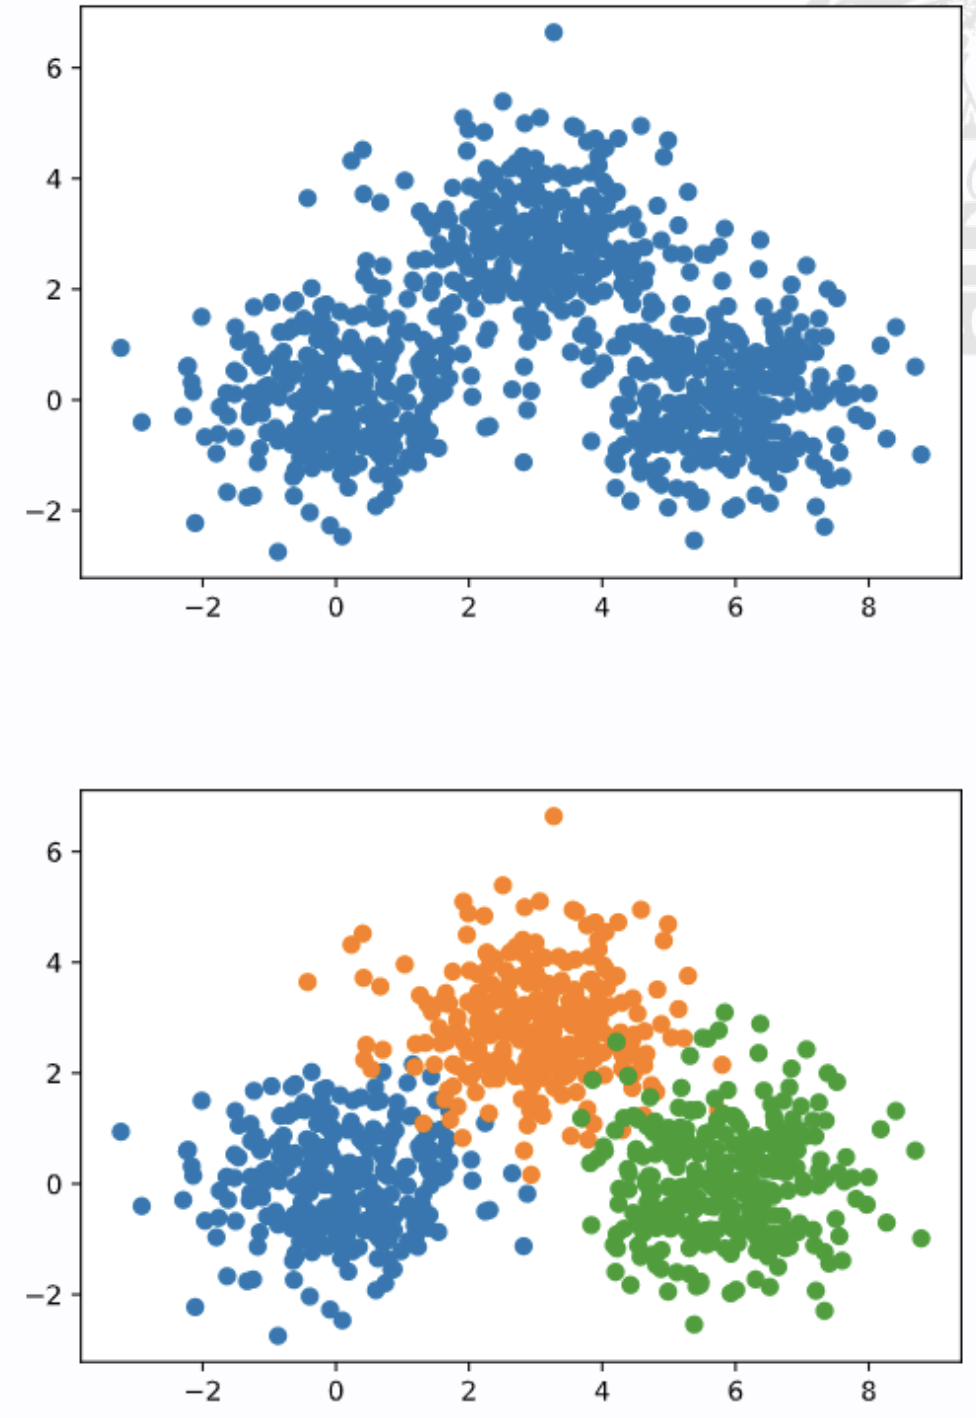
\includegraphics[scale=.3]{images/representation_learning/success.png}
  \centering
\end{figure}
\newpage
Se $h$ rappresenta tutti i fattori causali di $x$ e assumiamo che $y$ è correlato ad uno di essi, allora il
processo generativo può essere concepito come:
\begin{equation}
  p(h,x)=p(x|h)p(h)
\end{equation}
e i dati hanno probabilità marginale
\begin{equation}
  p(x)=\sum_hp(h,x)=\sum_hp(x|h)p(h)=\mathbb{E}_h[p(x|h)].
\end{equation}
Il miglior modello possibile di $x$ è quello che svela la struttura "vera" di cui sopra, con $h$ variabile
latente che spiega le variazioni osservate in $x$. Il punto è che calcolare l'expectation è difficile 
perchè non conosciamo $h$. Ma ammesso che conoscessimo il modo in cui calcolarla, nel mondo reale potrebbe 
essere comunque molto difficile. Quindi una domanda rilevante potrebbe essere: \textbf{quali sono i fattori 
causali importanti da considerare?} 
\newline
\newline
\paragraph{Come scegliere fattori causali da considerare?}
Molto spesso \textbf{la maggior parte delle osservazioni sono formate da un numero estremamente elevato di 
cause sottostanti}, l'approccio brute force di codificare tutti i possibili fattori di variazione non 
funziona: ad esempio in una scena visiva, la rappresentazione dovrebbe sempre codificare tutti gli oggetti?
Anche più piccoli sullo sfondo?


È quindi necessario decidere cosa codificare in $h$, ovvero trovare una strategia per guidare la rete a 
mantenere solo la parte \textbf{rilevante} di $h$.
Due strategie principali:
\begin{itemize}
  \item utilizzare un segnale supervisionato per guidare il processo non supervisionato;
  \item utilizzare un $h$ molto più grande quando si utilizza solo l'apprendimento non supervisionato.
\end{itemize}


\paragraph{Scegliere cosa codificare.}
Un'altra strategie emergente è quella del \textbf{cambiamente della definizione di cosa sia saliente}.
Storicamente, si ottimizzerebbe rispetto a un criterio fisso, spesso simile a \textbf{MSE (mean squared
error)}. Questo però potrebbe essere problematico.


Per esempio, la MSE applicata ai pixel di una immagine (object recognition), specicifica implicitamente 
che una causa è rilevante solo se influisce sulla luminosità di un gran numero di pixel. Più in generale, 
risulterebbero importanti solo i valori che causano una variazione di qualche tipo. 
\newline
\newline
Nell'immagine seguente, per sempio, l'oggetto sarebbe troppo piccolo da ricostruire. Ne consegue che 
abbiamo bisogno di altre tecniche, più complesse, per individuare i fattori.


\begin{figure}[!h]
  \centering
  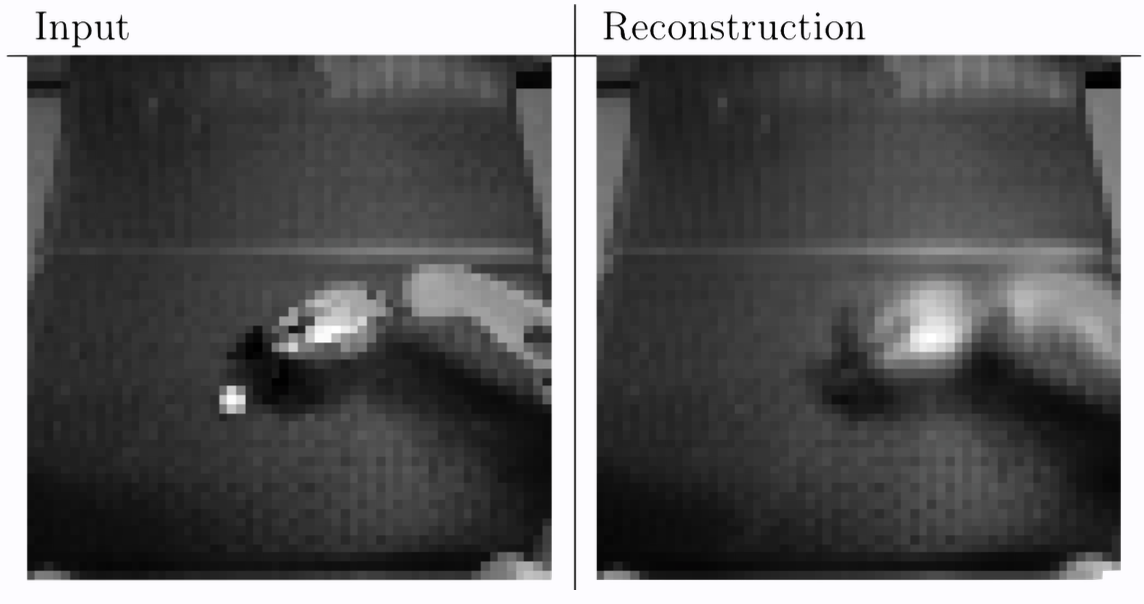
\includegraphics[scale=.4]{images/representation_learning/encode.png}
  \caption{Un autoencoder allenato con MSE per un task robotico ha fallito nel ricostruire la pallina da
  ping pong.}
\end{figure}
\newpage
E' in realtà possibile definire la salienza anche in altri modi.
\newline
Ad esempio, se un gruppo di pixel segue uno schema altamente riconoscibile, anche se tale schema non implica
un'estrema luminosità o oscurità, allora quello schema potrebbe essere considerato estremamente saliente.
\newline
Un modo per implementare tale definizione di salienza è utilizzare \textbf{generative adversarial networks
(GAN)}. Nelle GAN la salienza è definita implicitamente da un \textbf{gioco} tra un codificatore che cerca 
di ingannare e un discriminatore che cerca di indovinare.

\subsection{I fattori causali sono robusti}
Molto spesso, quando si considerano cambiamenti nella distribuzione dovuti a diversi domini, alla non 
stazionarietà temporale, o quando cambia la natura del task, \textbf{i meccanismi causali rimangono invariati} 
(le leggi dell'universo sono costanti) mentre la distribuzione marginale sulle cause sottostanti può cambiare.
\newpage
\section{Rapresentazioni Distribuite}
Un aspetto interessante delle reti neurali è che spesso apprendono rappresentazioni distribuite dei dati.
\newline
Una \textbf{rappresentazione distribuita} è una rappresentazione in cui ogni oggetto è descritto da molte
caratteristiche e ciascuna caratteristica è coinvolta nella rappresentazione di molti oggetti.
\newline
\newline
\textbf{Esempio:} consideriamo il caso di un sistema che ha bisogno di apprendere i colori e le forme di certi
oggetti:
\begin{itemize}
  \item colori $\in\{\text{red,green,blu}\}$;
  \item oggeti $\in\{\text{square,circle,triangle}\}$.
\end{itemize}
\begin{figure}[!h]
  \centering
  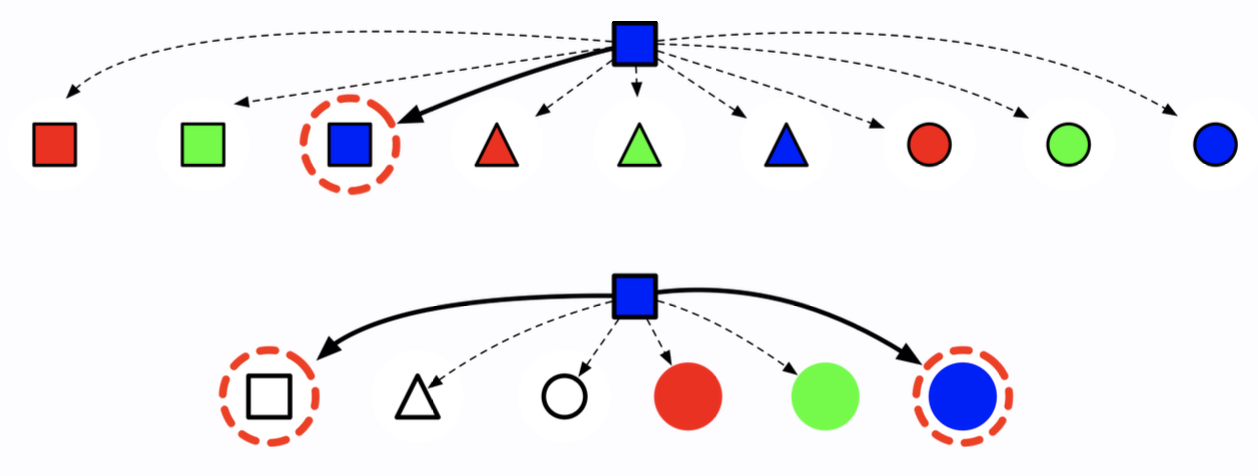
\includegraphics[scale=.5]{images/representation_learning/example01.png}
\end{figure}


Le rappresentazioni distribuite inducono un ricco similarity space, in cui concetti (o input) semanticamente 
vicini sono vicini anche dal punto di vista della distanza nello spazio, una proprietà che è assente nelle 
rappresentazioni puramente simboliche.


Esempio: "gatto" e "cane" come simboli sono distanti quanto qualsiasi altra coppia di simboli. Se vengono 
rappresentati con una rappresentazione distribuita, la rete tenderà a comprimere la rappresentazione in, per
il cane, "oggetto che ha due orecchie, quattro zampre eccetera". In questo modo, cane e gatto saranno in una
stessa zona nello spazio, che sarà però diversa dalla zona in cui si trova il trattore.
\newline
\newline
Inoltre, la rappresentazione distribuita aiuta a \textbf{rappresentare un numero esponenziale di regioni 
utilizzando un numero lineare di parametri}.
\begin{figure}[!h]
  \centering
  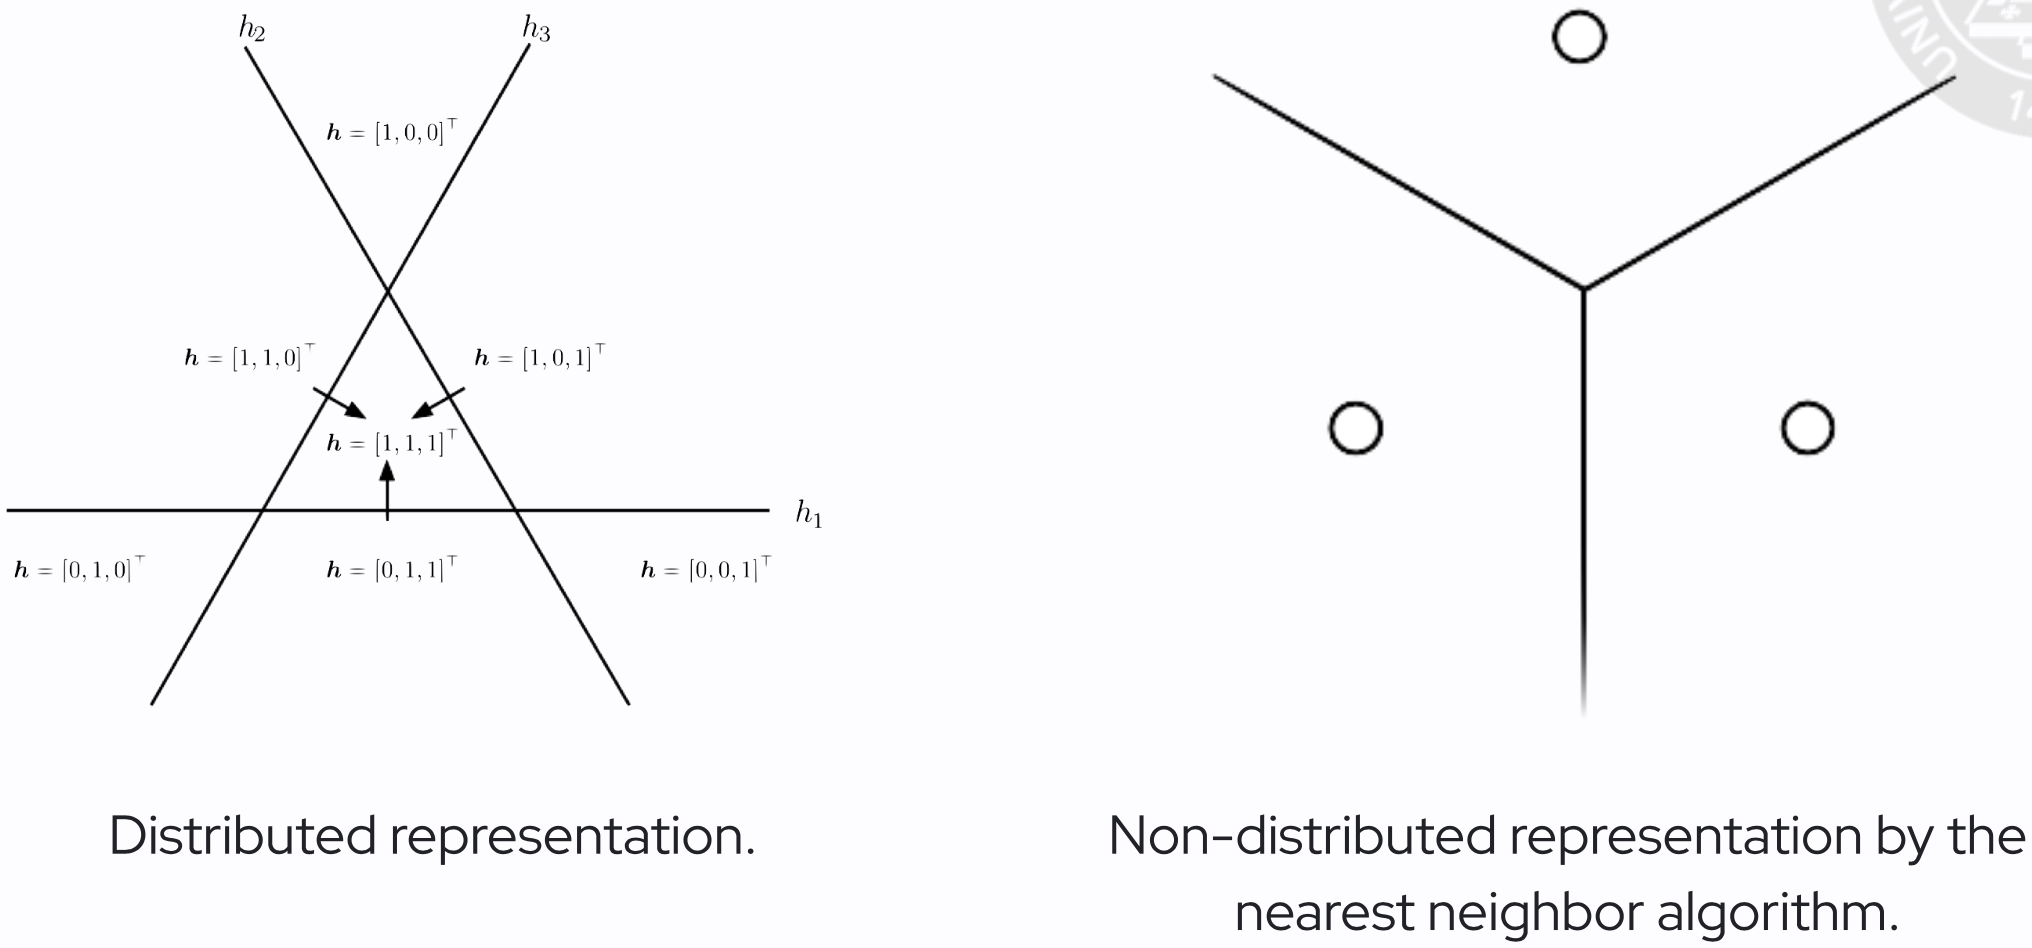
\includegraphics[scale=.5]{images/representation_learning/representation.png}
\end{figure}




